\documentclass{llncs}
\pdfoutput=1
% The following \documentclass options may be useful:
%
% 10pt          To set in 10-point type instead of 9-point.
% 11pt          To set in 11-point type instead of 9-point.
% authoryear    To obtain author/year citation style instead of numeric.

\usepackage{graphicx}
\usepackage{amsmath}
\usepackage{amssymb}
% \usepackage{amsthm}
\usepackage{array}
% \usepackage{cite}
\usepackage{hyperref}
\usepackage{listings}
\usepackage[nooneline,tight]{subfigure}
\usepackage[usenames,dvipsnames]{xcolor}
\usepackage{tikz}
\usepackage{booktabs}
\usepackage{microtype}
\usepackage{multirow}
\usepackage{flushend}
\usepackage{stmaryrd}
\usepackage[T1]{fontenc}
\usepackage{xspace}
\usepackage{xparse}
\usepackage{subdepth}
\usepackage{wrapfig}
\usepackage[inference]{semantic}
\usepackage{scalerel}

\usetikzlibrary{positioning,chains,shapes.arrows,shapes.geometric,fit,calc,arrows,decorations.pathmorphing}

\newcommand{\mynote}[2]{
  \textcolor{red}{%
    {\bfseries\sffamily\scriptsize#1}%
    {\small$\blacktriangleright$\textsf{\emph{#2}}$\blacktriangleleft$}}%
}

\newcommand{\todo}{\TODO}
\newcommand{\TODO}{\mynote}
\newcommand{\NOTE}{\mynote}

\newcommand{\TVar}[1]{#1^\ast}


\newcolumntype{C}[1]{>{\centering\arraybackslash}m{#1}} % zentrierte Spalten mit Breitenangabe 
\newcolumntype{P}[1]{>{\arraybackslash}m{#1}} % zentrierte Spalten mit Breitenangabe 
\newcommand{\mhline}{}

% \newtheorem{definition}{Definition}{\bfseries}{\itshape}
% \newtheorem{lemma}{Lemma}{\bfseries}{\itshape}
% \newtheorem{theorem}{Theorem}{\bfseries}{\itshape}
\newtheorem{innercustomthm}{Theorem}
\newenvironment{customtheorem}[1]
  {\renewcommand\theinnercustomthm{#1}\innercustomthm}
  {\endinnercustomthm}

% \newenvironment{itemize*}{%
%   \begin{itemize}\addtolength{\itemsep}{-.35\baselineskip}}{%
%   \end{itemize}}
% \newenvironment{enumerate*}{%
%   \begin{enumerate}\addtolength{\itemsep}{-.35\baselineskip}}{%
%   \end{enumerate}}
% \newenvironment{description*}{%
%   \begin{description}\addtolength{\itemsep}{-.35\baselineskip}}{%
%   \end{description}}

\newcommand{\sm}[1]{{\small #1}}

\makeatletter
\newcommand*{\mycleardoublepage}{\clearpage\if@twoside
\ifodd\c@page
  \hbox{}
%  \thispagestyle{empty}
  \clearpage
\fi
\hbox{}
\thispagestyle{empty}
\clearpage
\fi}
\makeatother


\newcounter{MOPReqCounter}
\newcommand{\MOPrequirement}[1]{
\begin{list}{\bfseries (R\arabic{MOPReqCounter})}{
\addtocounter{MOPReqCounter}{1}
\setlength\labelwidth{\widthof{\textbf{(RM)}}}
\addtolength\leftmargin{1.5em}
\addtolength{\itemsep}{-.35\baselineskip}
}
\item #1
\end{list}
}


\newcommand\positive{\tikz{\path [draw, fill] circle (0.7ex);}}
\newcommand\negative{\tikz{\path [draw] circle (0.7ex);}}
\newcommand\mixed{\tikz{\path [draw] (0,0) arc (0:180:0.7ex); \path [draw, fill] (0,0) arc (360:180:0.7ex);}}



%%%%%%%%%%%%%%%%%%%%
%% subfigure hackery
%%%%%%%%%%%%%%%%%%%%

% \captionsetup[subfigure]{labelfont=normal}

% lists
\makeatletter
\def\list@empty#1{}
\def\list@add#1#2{\edef#1##1{#1{##1}##1{#2}}}
\def\list@iterate#1#2{#1{#2}}
\makeatother

% subfigure environment
% (adapted from the subfigure package's documentation, section 4.7.4).

\makeatletter
\let\sfoldsubfigure=\subfigure
\let\sf@oldsubfigure=\subfigure
\let\subfigure=\thisisnotdefined
\let\sfenv@beginSubfigure=\relax
\let\sfenv@endSubfigure=\relax
\let\sfenv@beforeSubfigure=\relax
\let\sfenv@afterSubfigure=\relax
\newbox\subfigbox % Create a box to hold the subfigure.
\newenvironment{subfigure}% % Create the new environment.
{\def\caption##1{\gdef\subcapsave{\relax##1}}%
\let\subcapsave=\@empty % Save the subcaption text.
\let\sf@oldlabel=\label
\def\label##1{\global\list@add{\sublabsave}{##1}}
\let\sublabsave\list@empty % Save a list of label keys.
\setbox\subfigbox\hbox\bgroup\sfenv@beginSubfigure}% % Open the box...
{\sfenv@endSubfigure\egroup % ... close the box and call \subfigure.
\let\label=\sf@oldlabel
\sfenv@beforeSubfigure%
\sf@oldsubfigure[\subcapsave\list@iterate\sublabsave\label]{\box\subfigbox}}%
\sfenv@afterSubfigure%
\makeatother

% horizontal environment
% (to produce two columns of subfigures}

\makeatletter
\newenvironment{horizontal}
{\def\sfenv@beginSubfigure{\begin{minipage}{0.45\linewidth}}
\def\sfenv@endSubfigure{\end{minipage}}
\def\sfenv@beforeSubfigure{\hfil}
\def\sfenv@afterSubfigure{\hfil}}%
{\hfil}
\makeatother

% horizontal environment
% (to produce three columns of subfigures}

\makeatletter
\newenvironment{threecolumns}
{\def\sfenv@beginSubfigure{\begin{minipage}[b]{0.30\linewidth}}
\def\sfenv@endSubfigure{\end{minipage}}
\def\sfenv@beforeSubfigure{\hfil}
\def\sfenv@afterSubfigure{\hfil}}%
{\hfil}
\makeatother


% vertical environment
% (to produce rows of subfigures}

\makeatletter
\newenvironment{vertical}
{\def\sfenv@beginSubfigure{\begin{minipage}{\linewidth}}
\def\sfenv@endSubfigure{\end{minipage}}
\def\sfenv@beforeSubfigure{}
\def\sfenv@afterSubfigure{}}%
{}
\makeatother


%%%%%%%%%
%% colors
%%%%%%%%%

% \definecolor{myblue}{cmyk}{.8,.4,0,0}
% \definecolor{myred}{cmyk}{0,.95,.9,0}
% \definecolor{mypurple}{cmyk}{.3,.0,.3,0}
\colorlet{myblue}{blue}
\colorlet{myred}{red}
\colorlet{mypurple}{violet!150!black}
\colorlet{mygreen}{green!40!black}
\newcommand{\textblue}{\textcolor{myblue}}
\newcommand{\textred}{\textcolor{myred}}
\newcommand{\textpurple}{\textcolor{mypurple}}
\newcommand{\textgreen}{\textcolor{mygreen}}


\newenvironment{indented}[1][]%
{\noindent
 \begin{itemize}
 \item[#1]}%
{\end{itemize}}

\newcommand{\designGoal}[2]{%
  \begin{indented}
    \textit{#1}: #2%
  \end{indented}
}

\newcounter{goal}{}
\setcounter{goal}{0}
\newcommand{\getGoal}[1][\arabic{goal}]{\textbf{(DG#1)}}
\newcommand{\nextGoal}{%
  \addtocounter{goal}{1}%
  \getGoal}


%%%%%%%%%%%%%%%
%% case studies
%%%%%%%%%%%%%%%

\newenvironment{casestudy}{%
\ifx \restwidth \undefined
  \newlength{\restwidth}
\fi
\ifx \parparindent \undefined
  \newlength{\parparindent}
\fi
\setlength{\parparindent}{\parindent}
\setlength{\restwidth}{\linewidth}
\addtolength{\restwidth}{-\parindent}
%
\newcommand{\version}[1]{\colchunk{Version:}\colchunk{##1}\colplacechunks\vskip0.2em}
\newcommand{\developedBy}[1]{\colchunk{Developed by:}\colchunk{##1}\colplacechunks\vskip0.2em}
\newcommand{\size}[1]{\colchunk{Size:}\colchunk{##1}\colplacechunks\vskip0.2em}
\renewcommand{\description}[1]{\colchunk{Description:}\colchunk{##1}\colplacechunks\vskip0.2em}
\newcommand{\result}[1]{\colchunk{Results:}\colchunk{##1}\colplacechunks}
%
\renewcommand{\indent}{\hskip\parparindent}
%
\begin{parcolumns}[colwidths={1=0.17\linewidth},distance=1em]{2}
\parindent=0pt
}{%
\end{parcolumns}
}


%%% Local Variables: 
%%% mode: latex
%%% TeX-master: "document"
%%% End: 

\definecolor{keyword}{RGB}{96,0,53}
\definecolor{darkgreen}{RGB}{0,128,0}
\definecolor{listingsFrame}{gray}{0.6}

\newcommand{\fboxgray}[1]{%
    \colorlet{currentcolor}{.}%
    {\color{listingsFrame}%
    \fbox{\color{currentcolor}#1}}%
}

%%%%%%%%%%
%% styles
%%%%%%%%%%

\lstdefinestyle{normal}{%
  xleftmargin=\parindent,
}

\lstdefinestyle{nospace}{%
  aboveskip=0em,
  belowskip=0em,
  xleftmargin=0em,
  xrightmargin=0em,
%  basicstyle=\tiny\sf,
}

\lstdefinestyle{nohspace}{%
  xleftmargin=0em,
  xrightmargin=0em,
}


\lstdefinestyle{scriptsize}{%
  basicstyle=\scriptsize\sf,
}

\lstdefinestyle{footnote}{%
  basicstyle=\footnotesize\sf,
}

\lstdefinestyle{figureframe}{%
  xleftmargin=0pt,
  frame=single,
  rulecolor=\color{listingsFrame},
  numbersep=6pt,
}
\lstdefinestyle{inlineframe}{%
  xleftmargin=2pt,
  xrightmargin=2pt,
  frame=single,
  rulecolor=\color{listingsFrame},
  numbersep=6pt,
}


%%%%%%%%%%%%
%% languages
%%%%%%%%%%%%

\newcommand{\mytilde}{%
  \texttt{\resizebox{.48em}{1ex}{\hbox{$\sim$}}}%
}

\lstset{%
  columns=fullflexible,
  keepspaces=true,
  %basicstyle=\small\sf,
  basicstyle=\sffamily\small,
  % numberstyle=\tiny\ttfamily,
  showspaces=false,
  showstringspaces=false,
  style=normal,
  keywordstyle=\bfseries,
  stringstyle=\tt,% \color{blue}
  %commentstyle=\it\color{gray},
%
   literate={
    {˚}{{\texttt{\space}}}{1}
    {~}{{\mytilde}}{1}
    {=}{{\texttt{=}}}{1}
    {:}{{\texttt{:}}}{1}
    {-}{{\texttt{-}}}{1}
    {_}{{\texttt{\_}}}{1}
    {<}{{\texttt{<}}}{1}
    {>}{{\texttt{>}}}{1}   
    {+}{{\texttt{+}}}{1} 
    {*}{{\texttt{*}}}{1}
 %   {/}{{\texttt{/}}}{1}
    {|}{{\texttt{|}}}{1}
    {\&}{{\texttt{\&}}}{1}
   },
%  escapechar=\%,
  escapeinside={(@*}{*@)}
}
\newcommand{\lststring}[1]{{\tt\color{blue} #1}}
\newcommand{\lstmeta}[1]{{\it\color{darkgreen} #1}}

\lstdefinelanguage{LaTeX}[]{Tex}{%
  language=Tex,
  morekeywords={emph, label, ref, begin, end, part, chapter, section,
                subsection, subsubsection, paragraph, subparagraph, cite},
}


\lstdefinelanguage{SugarJ}[]{Java}{%
  language=Java,
  morekeywords={sugar, extension, context, free, syntax, desugarings, sorts, signature,
    constructors, rules, strategies, assert, as, editor, services, colorer, folding,
    outliner, checks, recursive, errors, warnings, where,
    css, outlining, rec, color, completions, completion, template,
    layout, analyses, then},
  mathescape=true,
  deletestring=[b]',
  morecomment=[l]{//},
}

\lstdefinelanguage{SugarJXML}[]{SugarJ}{%
  deletecomment=[l]{//},
  morecomment=[s]{<!--}{-->}
}

\lstdefinelanguage{SugarMDD}[]{SugarJ}{%
  morekeywords={model, transformation},
}

\lstdefinelanguage{SugarJATM}[]{SugarMDD}{%
  morekeywords={statemachine, initial, state, events},
}

\lstdefinelanguage{SugarJEntity}[]{SugarMDD}{%
  morekeywords={entity},
}
\lstdefinelanguage{SugarJATMEntity}[]{SugarJATM}{%
  morekeywords={data, entity},
}

\lstdefinelanguage{SugarJTemplate}[]{SugarMDD}{%
  morekeywords={in, \$for, template},
  mathescape=false
}

\lstdefinelanguage{SugarJFeature}[]{SugarMDD}{%
  morekeywords={featuremodel, features, constraint, config, enable, disable, variable},
  otherkeywords={\#ifdef},
}


\lstdefinelanguage{scala}{
  morekeywords={abstract,case,catch,class,def,%
    do,else,extends,false,final,finally,%
    for,if,implicit,import,match,mixin,%
    new,null,object,override,package,%
    private,protected,requires,return,sealed,%
    super,this,throw,trait,true,try,%
    type,val,var,while,with,yield},
%  otherkeywords={=>,<-,<\%,<:,>:,\#,@},
  sensitive=true,
  morecomment=[l]{//},
  morecomment=[n]{/*}{*/},
  morestring=[b]",
  morestring=[b]',
  morestring=[b]"""
}


\lstdefinelanguage{SDF}{%
  morekeywords={context, free, syntax, sorts, signature,
    constructors, rules, strategies, module, imports, exports},
  escapechar=_,
  mathescape=true,
  comment=[l]{\%\%},
  morestring=[b]",
}

\lstdefinelanguage{MyPython}[]{Python}{%
  escapechar=\%,
  mathescape=true,
}

\lstdefinelanguage{MyHaskell}[]{Haskell}{%
  escapechar=\%,
  mathescape=true,
  deletekeywords={Nothing,Just,False,True,putStrLn,fail,fromJust,lookup,Num,exp,free,snd,String,
  return,error,otherwise,not,show,read,Eval,Read,readsPrec,print},
}


\lstdefinelanguage{SugarHaskell}[]{MyHaskell}{%
  morekeywords={context, free, syntax, desugarings, sorts, signature,
    constructors, rules, strategies, lexical, reject},
  mathescape=false,
}

\lstdefinelanguage{SugarHaskellArrows}[]{SugarHaskell}{%
  morekeywords={proc},
}


\lstdefinelanguage{EBNF}{
  morestring=[b]"
}


\lstdefinelanguage{Constraint}{
% %  columns=spaceflexible,
%   literate={
%    {"}{{\texttt{"}}}{1}
%    {~}{{\texttt{ }}}{1}
%    {=}{{\texttt{=}}}{1}
%    {:}{{\texttt{:}}}{1}
%    {-}{{\texttt{-}}}{1}
%    {<}{{\texttt{<}}}{1}
%    {>}{{\texttt{>}}}{1}   
%    {+}{{\texttt{+}}}{1} 
%    {*}{{\texttt{*}}}{1}
%    {/}{{\texttt{/}}}{1}
%    {|}{{$\mid$}}{1}
%    {||}{{\texttt{||}}}{2}
%    {\&}{{\texttt{\&}}}{1}
%    {c}{{\it c}}{1}
%    {col}{{\texttt{col}}}{3}
%    {pmc}{pmc}{3}
%    {atomically}{atomically}{10}
%    {::=}{{\rm ::=}}{3}
%    {nat}{{\it number}}{6}
%   },
}


\lstdefinelanguage{Plain}{}

\lstdefinelanguage{Pseudo}{
  keywords={foreach,match,case,in,return,if,else},
  mathescape=true,
}

\lstdefinelanguage{Questionnaire}[]{Java}{%
  morekeywords = {questionnaire, question, value, Boolean, String, Integer, group,
    if, else, define, ask}
}

\newcommand{\lstplain}{\lstinline[language=Plain]}


%%% SugarFomega
\lstdefinelanguage{SugarFomega}{
  keywords = {module, val, type, mu, if, then, else, case, of,
    fold, unfold, true, false, as, public, import, syntax, desugaring, typing, context, free, let, in, end, forall, do},
  mathescape = true,
  morestring=[b]",
}
\newcommand{\sfo}{\lstinline[language=SugarFomega,basicstyle=\upshape\ttfamily\normalsize]}



%%% Local Variables: 
%%% mode: latex
%%% TeX-master: "document"
%%% End: 


\usetikzlibrary{positioning,chains,fit,calc,arrows,decorations.pathmorphing}
\usetikzlibrary{shapes.arrows,shapes.geometric,shapes.symbols}


%%%%%%%
%% tikz stuff
%%%%%%%


\tikzstyle{invisible} = []

\tikzstyle{model}
  = [ shape=rectangle
    , draw
    ]
\tikzstyle{transformation}
  = [ model
    , shape=single arrow
    , draw
    ]

\tikzstyle{meta} = [ double ]
\tikzstyle{generated} = [ dashed ]

\tikzstyle{mopdependency}
  = [ -stealth'
    , semithick
    ]
\tikzstyle{instance}
  = [ mopdependency
    , -open triangle 60
    ]

% Draws the outline of a bend arrow around a rectangle.
% 1. Parameter: name of the rectangle that contains the text
% 2. Parameter: head extend (use 0.25cm to fit with default tikz style)
% 3. Parameter: arc radius (again, 0.25cm seems to work well)
%
% This produces a path, so use it as follows:
%
% \draw[options here] \bendArrow{name of rectangle}{.25cm}{.25cm};
\newcommand{\bendArrow}[3]{
  let \p{content size} = ($(#1.north east) - (#1.south west)$) in
  let \n{tip length 1} = {veclen(0.5 * \y{content size}, 0.5 * \y{content size})} in
  let \n{tip length 2} = {veclen(#2,#2)} in

  (#1.north east)
  -- ++ (315 : \n{tip length 1})
  -- ++ (225 : \n{tip length 1} + \n{tip length 2})
  -- ++ (0, #2)
  -- (#1.south west)
  arc (270 : 180 : \y{content size} + #3)
  -- ++ (\y{content size}, 0)
  arc (180 : 270 : #3)
  (#1.north east)
  -- ++ (135 : \n{tip length 2})
  -- ++ (0, -#2)
  -- (#1.north west)}


%%%%%%%%%%%%%%%%%
%% diagram styles
%%%%%%%%%%%%%%%%%

\tikzstyle{document}
  = [ shape=rectangle
    , draw
    , minimum height=1.5em
    , text width=5em
    , text centered
    ]

\tikzstyle{component}
  = [ font=\scriptsize\it
    ]

\tikzstyle{code}
  = [ shape=rectangle
    , draw
    ]

\tikzstyle{process}
  = [ shape=single arrow
    , single arrow head extend=.75em
    , single arrow head indent=.25em
    , minimum width=3em
    , draw
    ]

\tikzstyle{point}
  = [ coordinate
    , minimum width=1em
    ]

\tikzstyle{flow diagram}
  = [ start chain
    , node distance=1em
    , every node/.style={on chain}
    ]

\tikzstyle{ast}
  = [ node distance=1em and 0.38em
    , every node/.style=ast node
    ]

\tikzstyle{ast node}
  = [ shape=circle
    , minimum size=0.5em
    , inner sep=0
    , fill
    ]

\tikzstyle{dependency}
  = [ dashed
    , -stealth'
    ]

\tikzstyle{red}
  = [ shape=rectangle
    , color=red
    ]

\tikzstyle{blue}
  = [ shape=circle
    , color=blue
    ]

\tikzstyle{green}
  = [ shape=diamond
    , color=green!80!black
    , minimum size=0.7em
    ]

\tikzstyle{note}
  = [ font=\scriptsize\it
    ]
    
\tikzstyle{zoomed arrow}
  = [ solid
    , decorate
    , decoration=snake
    , -stealth'
    ]

\tikzstyle{zoom}
  = [ dashed
    ]

\tikzstyle{uml class}
  = [ shape=rectangle
    , draw
    , font=\sf
    ]

\tikzstyle{uml package}
  = [ uml class
    , inner sep=1em
    ]

\tikzstyle{uml dependency}
  = [ dependency, 
    , dashed
%    , thick
    ]


\newcommand{\bluenode}{\tikz \node [ast node, blue, color=blue, text width=] {};}
\newcommand{\rednode}{\tikz \node [ast node, red, color=red, text width=] {};}
\newcommand{\greennode}{\tikz \node [ast node, green, color=green!80!black, text width=] {};}


\tikzstyle{double arrow}
  = [ shape=double arrow
    , double arrow head extend=.75em
    , double arrow head indent=.25em
    , minimum width=3em
    , draw
    , font=\sf
    ]

%% name graphs

\newdimen\nodedistance
\nodedistance=4em

\tikzstyle{name graph}
  = [ node distance=\nodedistance
    , every node/.style={namenode}
    , every path/.style={ref}
    ]


\tikzstyle{namenode}
  = [ circle
    , thick
    , anchor=center
    , draw
    , minimum size=2em
    , inner sep=2pt
    ]

\tikzstyle{synthesized}
  = [ namenode
    , fill=gray!45
    ]

\tikzstyle{ref}
  = [ -stealth'
    , semithick
    , draw
    ]

\tikzstyle{badref}
  = [ ref
    , dashed
    ]

%% expression trees

\newdimen\nodedistance
\nodedistance=4em

\tikzstyle{exp tree}
  = [ node distance=\nodedistance
    , every node/.style={exp node}
    , every path/.style={link}
    , execute at begin node={\strut}
    ]

\tikzstyle{exp node}
  = [ anchor=center
    ]
\tikzstyle{link}
  = [ semithick
    , draw
    ]

\tikzstyle{ctx node}
  = [ node distance = -.6em,
    ]
\tikzstyle{ctx edge}
  = [ color = myred
    , -stealth'
    ]

\tikzstyle{type node}
  = [ node distance = -.5em,
    ]
\tikzstyle{type edge}
  = [ color = myblue
    , -stealth'
    ]

%%%%%%%%%%%%%%%%%%%%%%%%%%%
% Pretty printing with tikz
%
% configuration

%%%%%%
%% TikZ and lstlistings
%%%%%%


% remembers a position on the page as a tikz coordinate
\newcommand{\coord}[1]{\tikz[remember picture] \coordinate (#1);}

% translation from baseline to upper border of box
\newcommand{\distanceTop}{7.15pt}

% translation from baseline to lower border of box
\newcommand{\distanceBottom}{-2.55pt}

% translation from baseline to left border of box
\newcommand{\distanceLeft}{-0.5pt}

% translation from baseline to right border of box
\newcommand{\distanceRight}{0.5pt}


% draws a rectangle around 2 points on the page
%
% optional parameter: TikZ style for the line
% 1. mandatory parameter: upper left corner, at text baseline height
% 2. mandatory parameter: lower right corner, at text baseline height
% 3. mandatory parameter: extra margin in all directions
\newcommand{\drawrect}[4][]{\begin{tikzpicture}[remember picture, overlay]
\draw[layout box, #1]
  ($(#2) +(\distanceLeft, \distanceTop) + (-#4, #4)$) rectangle
  ($(#3) + (\distanceRight, \distanceBottom) + (#4, -#4)$);
\end{tikzpicture}}

% draws a rectangle around 2 points on the page
%
% optional parameter: TikZ style for the line
% 1. mandatory parameter: left-hand-side of the first line, at text baseline height
% 2. mandatory parameter: a point on the left side of the rectangle
% 3. mandatory parameter: lower right corner, at text baseline height
% 4. mandatory parameter: extra margin in all directions
\newcommand{\drawbox}[5][]{\begin{tikzpicture}[remember picture, overlay]
\draw[layout box, #1]
  ($(#2) + (\distanceLeft, \distanceTop) + (-#5, #5)$) --
  ($(#4 |- #2) + (\distanceRight, \distanceTop) + (#5, #5)$) --
  ($(#4) + (\distanceRight, \distanceBottom) + (#5, -#5)$) --
  ($(#3 |- #4) + (\distanceLeft, \distanceBottom) + (-#5, -#5)$) --
  ($(#3 |- #2) + (\distanceLeft, \distanceBottom) + (-#5, -#5)$) --
  ($(#2) + (\distanceLeft, \distanceBottom) + (-#5, -#5)$) --
  cycle;
\end{tikzpicture}}

% draws a small \ppBox with three rows around the current point
% #1 = first.col
% #2 = left.col
% #3 = right.col
% #4 = last.col
\newcommand{\drawMiniBox}[4]{
  +(#2 * .2em, 0) --
  +(#2 * .2em, 1ex) --
  +(#1 * .2em, 1ex) --
  +(#1 * .2em, 1.5ex) --
  +(#3 * .2em, 1.5ex) --
  +(#3 * .2em, .5ex) --
  +(#4 * .2em, .5ex) --
  +(#4 * .2em, 0) --
  cycle
}

% A small box (for use inside text)
% optional argument = path options
% #1 = first.col
% #2 = left.col
% #3 = right.col
% #4 = last.col
\newcommand{\minibox}[5][]{%
  \begin{tikzpicture}[baseline=0pt]
  \path [mini layout box, #1]
    (0, 0) \drawMiniBox{#2}{#3}{#4}{#5};
  \end{tikzpicture}}

\newcommand{\miniboxA}{\minibox{-1}{0}{3}{3}}
\newcommand{\miniboxB}{\minibox{0}{0}{3}{3}}
\newcommand{\miniboxC}{\minibox{1}{0}{3}{3}}

% A small rectangle (for use inside text)
\newcommand{\minirect}{\hbox to 9pt{\drawrect[thin,scale=0.3,black]{0pt, 15pt}{26pt, -5pt}{0pt}}}


\tikzstyle{layout box}
  = [ blue
    % , semitransparent
    , semithick
    , draw
    ]

\tikzstyle{mini layout box}
  = [ black
    , very thin
    , draw
    ]

\tikzstyle{annotation}
  = [ font=\small\it
    ]

\tikzstyle{code annotation}
  = [ font=\small\it
    ]


% the font used for pretty printing
\newcommand{\selectCodeFont}{\sf\small}

% the font used for highlighting keywords
\newcommand{\selectKeywordFont}{\bfseries}

% the font used for highlighting string literals
\newcommand{\selectStringLitFont}{\tt}

% the font used for highlighting identifiers
\newcommand{\selectIdentifierFont}{\relax}

% the font used for highlighting operators
\newcommand{\selectOperatorFont}{\tt}

% the text height of token nodes
\newcommand{\tokenHeight}{2ex}

% the text depth of token nodes
\newcommand{\tokenDepth}{.5ex}

%%%%%%%%%%%%%%%%%%%%%%%%%%%
% Pretty printing with tikz
%
% tikz layer

% style for paths or scopes that do pretty printing
\tikzstyle{pretty print}
  = [ start chain=going base right
    , text height=\tokenHeight
    , text depth=\tokenDepth
    , inner sep=0
    , node distance=0em
    ]

% helper style for nodes that start a new line
% (automatically applied by style 'new line' below)
\tikzstyle{new line/helper}
  = [ on chain
    , anchor=north west,
      at={($(#1.west |- \tikzchainprevious.base) + (0, -1.1\baselineskip)$)}
    ]

\tikzstyle{new line tight/helper}
  = [ on chain
    , anchor=north west,
      at={($(#1.west |- \tikzchainprevious.base) + (0, -0.9\baselineskip)$)}
    ]


% style for nodes that start a new line
\tikzstyle{new line}[\tikzchainprevious]
  = [ on chain=placed {new line/helper=#1}
    ]

% style for nodes that start a new line
\tikzstyle{new line tight}[\tikzchainprevious]
  = [ on chain=placed {new line tight/helper=#1}
    ]

% helper style for nodes that tab forward to a labeled position
% (automatically applied by style 'tab forward' below)
\tikzstyle{tab forward/helper}
  = [ on chain
    , anchor=north west,
      at={(#1 |- \tikzchainprevious.base)}
    ]

% style for nodes that tab forward to a labeled position
\tikzstyle{tab forward}
  = [ on chain=placed {tab forward/helper=#1}
    ]

% style for nodes that indent
\tikzstyle{indent}[1em]
  = [ on chain=placed {base right=#1 of \tikzchainprevious}
    ]

% style for nodes that contain an identifier token
\tikzstyle{identifier}
  = [ on chain
    , font=\selectIdentifierFont
    ]

% style for nodes that contain an operator token
\tikzstyle{operator}
  = [ on chain
    , font=\selectOperatorFont
    ]

% style for nodes that contain a keyword token
\tikzstyle{keyword}
  = [ on chain
    , font=\selectKeywordFont
    , text=keyword
    ]

% style for nodes that contain a string literal
\tikzstyle{stringlit}
  = [ on chain
    , font=\selectStringLitFont
    , text=blue
    ]

%%%%%%%%%%%%%%%%%%%%%%%%%%%
% Pretty printing with tikz
%
% \ppBox layer

\newcommand{\Empty}{}
\newcommand{\ignore}[1]{\relax}

\makeatletter
\newcommand{\ppBox}[2][]{{
  % insert keyword token
  \newcommand{\KW}[1]{
    \node[keyword] {##1};
    \HandleToken{\tikzchaincurrent}}

  % insert identifier token
  \newcommand{\ID}[1]{
    \node[identifier] {##1};
    \HandleToken{\tikzchaincurrent}}

  % insert operator token
  \newcommand{\OP}[1]{
    \node[operator] {##1};
    \HandleToken{\tikzchaincurrent}}

  % insert whitespace token
  \newcommand{\SP}{
    \node[on chain] { };
    \HandleInsensitiveToken{\tikzchaincurrent}}

  % label a position (with a tikz node name)
  \newcommand{\LB}[1]{
    \coordinate[on chain] (##1);}

  % tab forward to a labeled position
  \newcommand{\TB}[1]{
    \coordinate[tab forward=##1];
  }

  % insert a string literal
  \newcommand{\STR}[1]{
    \node[stringlit] {##1};
    \HandleToken{\tikzchaincurrent}}

  % insert a line break
  \renewcommand{\\}{
    \coordinate[new line=\NewlineNode];
    \let\HandleToken=\HandleTokenSubsequentLine}

  \newcommand{\newlineTight}{
    \coordinate[new line tight=\NewlineNode];
    \let\HandleToken=\HandleTokenSubsequentLine}

  % the name of the first token
  \let\FirstToken=\Empty
  \newcommand{\AdjustFirst}[1]{
    \ifx\FirstToken\Empty
    \edef\FirstToken{##1}
    \fi
  }

  % the name of the last token
  \let\LastToken=\Empty
  \newcommand{\AdjustLast}[1]{
    \edef\LastToken{##1}
  }

  % the name of the left-most token
  % (except for tokens in the first line)
  \let\LeftToken=\Empty
  \newcommand{\AdjustLeft}[1]{
    \ifx\LeftToken\Empty
      \edef\LeftToken{##1}
    \else
      \pgf@process{\pgfpointanchor{##1}{west}}
      \setlength{\pgf@xa}{\pgf@x}
      \pgf@process{\pgfpointanchor{\LeftToken}{west}}
      \setlength{\pgf@xb}{\pgf@x}
      \ifdim\pgf@xa<\pgf@xb
        \edef\LeftToken{##1}
      \fi
    \fi
  }

  % the name of the rightmost token
  \let\RightToken=\Empty
  \newcommand{\AdjustRight}[1]{
    \ifx\RightToken\Empty
      \edef\RightToken{##1}
    \else
      \pgf@process{\pgfpointanchor{##1}{east}}
      \setlength{\pgf@xa}{\pgf@x}
      \pgf@process{\pgfpointanchor{\RightToken}{east}}
      \setlength{\pgf@xb}{\pgf@x}
      \ifdim\pgf@xa>\pgf@xb
        \edef\RightToken{##1}
      \fi
    \fi
  }

  % this is called for all layout-sensitive tokens in the first
  % line of a pretty printing group
  \newcommand{\HandleTokenFirstLine}[1]{
    \AdjustFirst{##1}
    \AdjustRight{##1}
    \AdjustLast{##1}
  }

  % this is called for all layout-sensitive tokens in subsequent
  % lines of a pretty printing group
  \newcommand{\HandleTokenSubsequentLine}[1]{
    \AdjustLeft{##1}
    \AdjustRight{##1}
    \AdjustLast{##1}}

  % this is called for layout-insensitive tokens in a pretty
  % printing group (such as whitespace, comments, and code that
  % uses explicit layout)
  \newcommand{\HandleInsensitiveToken}[1]{
  }

  % current token handler. will be set to one of:
  %  \HandleTokenFirstLine
  %  \HandleTokenSubsequentLine
  %  \HandleInsensitiveToken
  \newcommand{\HandleToken}[1]{}

  \newcommand{\ppSubBox}[2][]{
    \coordinate[on chain];
    {
      \let\NewlineNode\tikzchaincurrent

      % reset the token registers
      \let\FirstToken=\Empty
      \let\LastToken=\Empty
      \let\LeftToken=\Empty
      \let\RightToken=\Empty

      % start in first line
      \let\HandleToken=\HandleTokenFirstLine

      % typeset content
      ##2

      % draw boundary
      \ifx\LeftToken\Empty
        \path [##1]
          (\FirstToken.north west) rectangle
          (\LastToken.south east);
      \else
        \path [##1]
          (\RightToken.east |- \FirstToken.north) --
          (\FirstToken.north west) --
          (\FirstToken.south west) --
          (\LeftToken.west |- \FirstToken.south) --
          (\LeftToken.west |- \LastToken.south) --
          (\LastToken.south east) --
          (\LastToken.north east) --
          (\RightToken.east |- \LastToken.north) --
          cycle;
      \fi

      % remember the token registers outside the group
      \global\let\InnerFirstToken=\FirstToken
      \global\let\InnerLastToken=\LastToken
      \global\let\InnerLeftToken=\LeftToken
      \global\let\InnerRightToken=\RightToken

      % remember the state outside the group
      \global\let\InnerHandleToken=\HandleToken
    }
    % handle the significant inner tokens
    % and significant inner linebreaks
    \HandleToken{\InnerFirstToken}
    \ifx\HandleToken\HandleTokenFirstLine
    \let\HandleToken=\InnerHandleToken
    \fi
    \ifx\InnerLeftToken\Empty
    \else
    \HandleToken{\InnerLeftToken}
    \fi
    \HandleToken{\InnerRightToken}
    \HandleToken{\InnerLastToken}
  }

  % indent a ppBox
  \newcommand{\IN}[1]{\coordinate[indent]; ##1}
  \newcommand{\DE}[1]{\coordinate[indent=-1em]; ##1}

  \let\ppBox=\ppSubBox
  \ppBox[#1]{#2}}}
\makeatother




%%% Local Variables: 
%%% mode: latex
%%% TeX-master: "document"
%%% End: 


\newif\iftechreport
%\techreporttrue % uncomment to activate tech-report setup
\techreportfalse % uncomment to deactivate tech-report setup

\newcommand{\proofsketch}[1]{{\def\proofname{Proof sketch}\proof{#1}}}

% this are the defaults from article.cls
\renewcommand\floatpagefraction{.9}
\renewcommand{\topfraction}{.9}
\renewcommand{\bottomfraction}{.1}
\renewcommand\textfraction{.1}  

% \addtolength{\abovecaptionskip}{-0.4cm}
% \newcommand{\captionskip}{1.5ex}
% \addtolength{\belowcaptionskip}{-\captionskip}

\hyphenation{meta-lan-guage}
\hyphenation{meta-lan-guages}
\hyphenation{SugarJ}
\hyphenation{JastAddJ}
\hyphenation{name-space}
\hyphenation{name-space}

\begin{document}

\title{A Co-Contextual Formulation of Type Rules\\ and its Application to Incremental Type Checking}
% alternative titles: 
% Co-Contextual Type Rules for Incremental Type Checking
%

% \author{Authors omitted for double-blind review}
% \institute{}
\author{Sebastian Erdweg\and Oliver Bra\v{c}evac \and Edlira Kuci \newline Matthias
  Krebs \and Mira Mezini%
}
\institute{TU Darmstadt, Germany}

\maketitle

\begin{abstract}
  Type rules associate types to expressions given a typing context. As the type
  checker traverses the expression tree top-down, it extends the typing context
  with additional context information that becomes available. This way, the
  typing context coordinates type checking in otherwise independent
  subexpressions, which inhibits parallelization and incrementalization of type
  checking.

  We propose a co-contextual formulation of type rules that only take an
  expression as input and produce a type and a set of \emph{context
    requirements}. Co-contextual type checkers traverse an expression tree
  bottom-up and merge context requirements of independently checked
  subexpressions. We describe a method for systematically constructing a
  co-contextual formulation of type rules from a regular context-based
  formulation and we show how co-contextual type rules give rise to incremental
  type checking. Using our method, we derive incremental type checkers for PCF
  and for extensions that introduce references, parametric polymorphism, and
  subtyping. Our performance evaluation shows that co-contextual type checking
  has performance comparable to standard context-based type checking, and
  incrementalization can improve performance significantly.
\end{abstract}

\renewcommand{\paragraph}[1]{\vspace{1ex}\noindent\textbf{#1}}


\newcommand{\OR}{\ensuremath{\;|\;}}
\newcommand{\WHERE}{\OR}
\newcommand{\ctxcolor}{\textred}
\newcommand{\typecolor}{\textblue}
\newcommand{\conscolor}{\textblue}
\newcommand{\reqcolor}{\textred}
\newcommand{\typectxcolor}[1]{\textpurple{\ensuremath{#1}}}
\newcommand{\type}[1]{\ensuremath{\typecolor{#1}}}
\newcommand{\context}[1]{\ensuremath{\ctxcolor{#1}}}

\newcommand{\TNum}{\ensuremath{\mathit{Num}}\xspace}
\newcommand{\TRecord}[5]{\ensuremath{\{#1 \ofType #2\}_{#3 \in #4 \ldots #5}}}
\newcommand{\TFloat}{\ensuremath{\mathit{Float}}\xspace}
\newcommand{\TReal}{\ensuremath{\mathit{Real}}\xspace}
\newcommand{\TUniv}[2]{\ensuremath{\forall#1.\,#2}}
\newcommand{\ofType}{\ensuremath{\mathop{:}}}
\renewcommand{\to}{\mathop{\rightarrow}}
\newcommand{\ctxplus}[2]{\ensuremath{#1; #2}}
\newcommand{\coctxplus}[2]{#1; #2}
\newcommand{\dom}[1]{\textit{dom}(#1)}
\newcommand{\fvt}[1]{\textit{fv}(#1)}

\newcommand{\abs}[3]{\ensuremath{\lambda #1 \ofType #2.\ #3}}
\newcommand{\absNoType}[2]{\ensuremath{\lambda #1.\ #2}}
\newcommand{\tabs}[2]{\ensuremath{\lambda #1.\ #2}}
\newcommand{\tapp}[2]{\ensuremath{#1[#2]}}
\newcommand{\app}[2]{\ensuremath{#1\, #2}}
\newcommand{\fix}[1]{\ensuremath{\mathit{fix}\; #1}}
\newcommand{\add}[2]{\ensuremath{#1 \mathop{+} #2}}
\newcommand{\sub}[2]{\ensuremath{#1 \mathop{-} #2}}
\newcommand{\mul}[2]{\ensuremath{#1 \mathop{*} #2}}
\newcommand{\ifzero}[3]{\ensuremath{\mathit{if0}\; #1\; #2\; #3}}
\newcommand{\record}[5]{\ensuremath{\{#1 = #2\}_{#3 \in #4 \ldots #5}}}

\newcommand{\reqs}[0]{\ensuremath{R}}
\newcommand{\treqs}[0]{\ensuremath{R^T}}
\newcommand{\appNode}[0]{\textsf{app}\xspace}
\newcommand{\tappNode}[0]{\textsf{tapp}\xspace}
\newcommand{\absNode}[2]{\ensuremath{\lambda #1 \ofType #2}\xspace}
\newcommand{\ctxNode}[1]{\ensuremath{\ctxcolor{#1 \mathop{\vdash}}\, }}
\newcommand{\typeNode}[1]{\ensuremath{\,\typecolor{\mathop{:} #1}}}
\newcommand{\coctxNode}[1]{\ensuremath{\mathrel{|} \ctxcolor{#1}}}
\newcommand{\consNode}[1]{\ensuremath{\mathrel{|} \conscolor{#1}}}
\newcommand{\reqNode}[1]{\ensuremath{\mathrel{|} \reqcolor{#1}}}
\newcommand{\reqmerge}[2]{\ensuremath{\mathit{merge}(#1, #2)}}
\newcommand{\reqmergeF}[0]{\ensuremath{\mathit{merge}}\xspace}
\newcommand{\addNode}[0]{\ensuremath{\mathop{+}}}
\newcommand{\mulNode}[0]{\ensuremath{\mathop{*}}}
\newcommand{\subNode}[0]{\ensuremath{\mathop{-}}}
\newcommand{\ifzeroNode}[0]{\ensuremath{\mathit{if0}}\xspace}

\newcommand{\judge}[3]{\ensuremath{\ctxcolor{#1} \mathrel{\vdash} #2 \mathrel{:} \typecolor{#3}}}
\newcommand{\judgeC}[4]{\ensuremath{\ctxcolor{#1} \mathrel{\vdash} #2 \mathrel{:} \typecolor{#3} \mathrel{|} \typecolor{#4}}}
\newcommand{\cojudge}[4]{\ensuremath{#1 \mathrel{:} \typecolor{#2} \mathrel{|} \typecolor{#3} \mathrel{|} \ctxcolor{#4} }}
\newcommand{\cojudgePol}[5]{\ensuremath{#1 \mathrel{:} \typecolor{#2} \mathrel{|} \typecolor{#3} \mathrel{|} (\ctxcolor{#4},\ctxcolor{#5}) }}
\newcommand{\coTypeOK}[2]{\ensuremath{\vdash #1\ \textsf{ok}\mathrel{|} \ctxcolor{#2} }}
\newcommand{\mustEqual}[0]{\ensuremath{\overset{!}{=}}}
\newcommand{\rulename}[1]{\ensuremath{\textsc{\scriptsize #1}}\xspace}
\newcommand{\fresh}[1]{\ensuremath{\typecolor{#1}\ \textit{is fresh}}}

\newcommand{\smap}{\ensuremath{\mathop{\!\mapsto\!}}}
\newcommand{\subst}[2]{\ensuremath{\{#1\}}#2}
\newcommand{\CSubst}[4]{\ensuremath{{#1} \mathop{=} \{{#3}\smap{#4}\}{#2}}}

\newcommand{\consjoin}[3]{\ensuremath{#1 = #2 \vee #3}}
\newcommand{\joinop}[2]{\ensuremath{#1 \vee #2}}
\newcommand{\consmeet}[3]{\ensuremath{#1 = #2 \wedge #3}}
\newcommand{\meetop}[2]{\ensuremath{#1 \wedge #2}}
\newcommand{\subtpe}{\ensuremath{\mathbin{\!\scalerel{{<}\!}{\colon}\!\!}}}
\newcommand{\conssub}[2]{\ensuremath{#1 \subtpe #2 }}
\newcommand{\pcfsub}{\ensuremath{\text{PCF}_{\subtpe}}}

\newcommand{\annotateNode}[4]{\node[type node, right=of #1] (#1-type) {\typeNode{#2}};
  \node[ctx node, right=of #1-type] (#1-cons) {\consNode{#3}};
  \node[ctx node, right=of #1-cons] (#1-req) {\reqNode{#4}};}
\newcommand{\TNumeric}{\ensuremath{\mathit{Numeric}}\xspace}

\newcommand{\treegen}[3]{\mathit{T}({#1}^{#2},#3)}

\section{Introduction}
\label{sec:introduction}

Type checkers of modern programming languages play an important role in assuring software quality as they try to statically prove increasingly strong invariants over programs. 

Typically, a type checker starts processing at the root node of a syntax tree 
and takes a typing context as an additional input to coordinate between sub-derivations by assigning types to jointly used variables. 
While traversing down the tree, the type checker extends the context with
type bindings, making them available in subexpressions.
When the type checker reaches a variable, it looks up the corresponding binding
in the typing context. Since variables constitute leaves of the syntax tree, the
downward traversal ends. The type checker then propagates the derived types back
upward the syntax tree. In summary, while types flow bottom-up, typing contexts
flow top-down -- overall, the type system runs in a "down-up" mode.

The top-down context propagation of contexts has some problems. It hampers parallel, 
incremental type checking as well as compositional type checking 
%compilation and compositional explanation of 
because the typing of subexpressions depends on the
typing of parent expressions (to retrieve the context) and vice versa (to
retrieve the types). In this paper, we are specifically interested in incremental type checking. 
Type checking may take considerable time. Especially for large software systems, it is important to reduce the
run time of type checking to enable short feedback cycles~\cite{KuhnMT12}. To this end, some forms of incremental type checking find
increasing interest in industry and, for example, are used in Eclipse's JDT and
Facebook's Flow and Hack. 
%However, incrementalizing a type checker is difficult because the typing context coordinates between subderivations by assigning types to jointly used variables. 


To enable type checkers with fine-grained incrementalization, we propose to eliminate top-down propagated contexts and to replace them by the dual concept of bottom-up propagated \emph{context
requirements}. We call such a type checking \emph{co-contextual}. A co-contextual type
checker starts processing at the leaves. Instead of looking up variables in a context, it invents fresh type variables as placeholders for their actual types. In addition, the co-contextual type checker
generates context requirements that demand the variables are actually bound with
this type. As the co-contextual type checker progresses up the syntax
tree, it refines the types of subexpressions and merges their context requirements.

To give an intuition about our proposal, 
we consider the process of type checking the simply-typed expression
\abs{f}{\alpha\to\beta}{\abs{x}{\alpha}{\app{f}{x}}} ($\alpha$ and $\beta$
are arbitrary but fixed types) with an ordinary and a co-contextual  type checker.
The following figure depicts the ordinary type checking. 
It shows the syntax tree of the expression explicitly, marking the application term with
\appNode. We attach typing contexts and types to syntax tree nodes on
their left-hand and right-hand side, respectively. The type attached
to a node represents the type of the whole subexpression.
%
\begin{center}
\begin{tikzpicture}[exp tree]
  \node (lambda-f) at (0,4) {\absNode{f}{\alpha\to\beta}};
  \node (lambda-x) at (0,3) {\absNode{x}{\alpha}};
  \node (app) at (0,2) {\appNode};
  \node (f) at (-2.5,0.5) {$f$};
  \node (x) at (2.5,0.5) {$x$};

  \node[ctx node, left=of lambda-f]  (lambda-f-ctx)  {\ctxNode{\Gamma}};
  \node[type node, right=of lambda-f] (lambda-f-type) {\typeNode{(\alpha\to\beta) \to \alpha \to \beta}};
  \node[ctx node, left=of lambda-x]  (lambda-x-ctx)  {\ctxNode{\ctxplus{\Gamma}{f \ofType \alpha\to\beta}}};
  \node[type node, right=of lambda-x] (lambda-x-type) {\typeNode{\alpha \to \beta}};
  \node[ctx node, left=of app]  (app-ctx)  {\ctxNode{\ctxplus{\ctxplus{\Gamma}{f \ofType \alpha\to\beta}}{x \ofType \alpha}}};
  \node[type node,right=of app] (app-type) {\typeNode{\beta}};
  \node[ctx node, left=of f]  (f-ctx)  {\ctxNode{\ctxplus{\ctxplus{\Gamma}{f \ofType \alpha\to\beta}}{x \ofType \alpha}}};
  \node[type node,right=of f] (f-type) {\typeNode{\alpha\to\beta}};
  \node[ctx node, left=of x]  (x-ctx)  {\ctxNode{\ctxplus{\ctxplus{\Gamma}{f \ofType \alpha\to\beta}}{x \ofType \alpha}}};
  \node[type node,right=of x] (x-type) {\typeNode{\alpha}};

 \path (lambda-f) edge (lambda-x);
 \path (lambda-x) edge (app);
 \path (app) edge (f);
 \path (app) edge (x);

\node (ctx-flow-top) at (-4,4) {};
\node (ctx-flow-bot) at (-4,.5) {};
\draw[ctx edge] (ctx-flow-top) -- (ctx-flow-bot) node[left,pos=.5,align=right] {\ctxcolor{contexts} flow\\ top-down};

\node (type-flow-bot) at (3,4) {};
\node (type-flow-top) at (3,.5) {};
\draw[type edge] (type-flow-top) -- (type-flow-bot) node[right,pos=.5,align=left] {\typecolor{types} flow\\ bottom-up};
\end{tikzpicture}
\end{center}
%

The following figure depicts the process of type checking the same expression by a co-contextual type checker. We separate a node's type $T$ and context requirements $\reqs$ by a
vertical bar $T\mathrel{|}\reqs$. The following tree illustrates how a co-contextual type check 
enables type checking a program bottom-up.

%
%
\begin{center}
\begin{tikzpicture}[exp tree]
  \node (lambda-f) at (0,4) {\absNode{f}{\alpha\to\beta}};
  \node (lambda-x) at (0,3) {\absNode{x}{\alpha}};
  \node (app) at (0,2) {\appNode};
  \node (f) at (-2.5,0.5) {$f$};
  \node (x) at (2.5,0.5) {$x$};

  \node[type node, right=of lambda-f] (lambda-f-type) {\typeNode{(\alpha\to\beta) \to \alpha \to \beta}};
  \node[ctx node, right=of lambda-f-type]  (lambda-f-ctx)  {\coctxNode{\emptyset}};
  \node[type node, right=of lambda-x] (lambda-x-type) {\typeNode{\alpha \to U_2}};
  \node[ctx node, right=of lambda-x-type]  (lambda-x-ctx)  {\coctxNode{f \ofType \alpha \to U_2}};
  \node[type node,right=of app] (app-type) {\typeNode{U_2}};
  \node[ctx node, right=of app-type]  (app-ctx)  {\coctxNode{\coctxplus{f \ofType U_1 \to U_2}{x \ofType U_1}}};
  \node[type node,right=of f] (f-type) {\typeNode{U_0}};
  \node[ctx node, right=of f-type]  (f-ctx)  {\coctxNode{f \ofType U_0}};
  \node[type node,right=of x] (x-type) {\typeNode{U_1}};
  \node[ctx node, right=of x-type]  (x-ctx)  {\coctxNode{x \ofType U_1}};

 \path (lambda-f) edge (lambda-x);
 \path (lambda-x) edge (app);
 \path (app) edge (f);
 \path (app) edge (x);

\node (type-flow-bot) at (4,4) {};
\node (type-flow-top) at (4,.5) {};
\draw[type edge] (type-flow-top) -- (type-flow-bot);

\node (ctx-flow-bot) at (4.2,4) {};
\node (ctx-flow-top) at (4.2,.5) {};
\draw[ctx edge] (ctx-flow-top) -- (ctx-flow-bot) node[right,pos=.5,align=left] {\typecolor{types} and \ctxcolor{contexts}\\ flow bottom-up};

\end{tikzpicture}
\end{center}
%

%\noindent We call such type checking \emph{co-contextual}. A co-contextual type
%checker starts processing at the leaves. Instead of looking up variables $f$ and
%$x$ in the context, we invent fresh type variables $U_0$ and $U_1$ as
%placeholders for their types. In addition, the co-contextual type checker
%generates context requirements that demand the variables are actually bound with
%this type. In the illustration, we separate a node's type $T$ and context requirements $\reqs$ by a
%vertical bar $T\mathrel{|}\reqs$. As the co-contextual type checker progresses up the syntax
%tree, it refines the types of subexpressions and merges their context requirements.

For the application term, the type checker refines $U_0$ to be a function type
from $U_1$ to a fresh type variable $U_2$, which becomes the result type of the
application term. Next, the type checker collects all context requirements of
subexpressions, applies the type refinements to them, and propagates them
upward. This changes the type of $f$ in the requirements. A
$\lambda$-abstraction eliminates context requirements on the bound
variable. When reaching the $\lambda$-abstraction of $x$, the type checker
matches the required type for $x$ with the declared type of $x$ and 
propagates only the remaining requirement on $f$ upward. Finally,
the co-contextual type checker finds the same type as the context-based type
checker above, and all context requirements have been satisfied. Any remaining
context requirements in the root node of a program indicate a type error.

To see how co-contextual type checking avoids contextual coordination, consider
the program \abs{x}{U_0}{\app{x}{x}}. A context-based type checker propagates a
single context \ctxplus{\Gamma}{x \ofType U_0} to all subexpressions of the
$\lambda$-abstraction, thus making sure that $U_0$ is used consistently as the type
of $x$. In contrast, a co-contextual type checker generates context requirements
$x \ofType U_1$ and $x \ofType U_2$ for the two variable nodes
independently. Only when merging these requirements in the application term
\app{x}{x}, the type checker coordinates the type of $x$ by refining $U_1 =
U_2$. In our example, this leads to a type error because type checking
the application term also refines $U_1$ to a function type $U_2 \to U_3$. Thus,
the type checker derives the unsolvable constraint $U_2 = U_2 \to U_3$ and
correctly indicates a type error.

Since co-contextual type checkers do not coordinate subderivations, it is
possible to incrementalize them systematically by applying memoization,
incremental constraint solving, and eager substitution. Such incrementalization
is independent of the module structure of the program. \\

\noindent
In summary, we make the
following contributions:

\begin{itemize}
\item We describe a method for constructing co-contextual type rules from
  traditional context-based type rules.
\item We derive co-contextual type systems for PCF and for extensions that
  handle records, parametric polymorphism, and subtyping.
\item We describe how co-contextual type systems give rise to incremental type
  checking, given that the type rules are in algorithmic form.
\item We explain how to implement incremental type checking efficiently and
  describe implementations for PCF and its extensions.
\item We evaluate the non-incremental and incremental performance of the
  co-contextual PCF type checker by comparison to a context-based algorithm.
\end{itemize}

%==== previous version ===

%Type checkers of modern programming languages try to prove increasingly strong
%invariants over a program and take considerable time~\cite{type checkers are
%slow}. Especially for large software systems, it is important to reduce the
%run time of type checking to enable short feedback cycles~\cite{feedback cycles
%  are important}. To this end, forms of incremental type checking find
%increasing interest in industry and, for example, are used in Eclipse's JDT and
%Facebook's Flow and Hack. However, incrementalizing a type checker is difficult
%because the typing context coordinates between subderivations by assigning types
%to jointly used variables. We propose a technique for eliminating contextual
%coordination in order to derive type checkers with fine-grained
%incrementalization.

%To illustrate our technique, let us first investigate how an ordinary type
%checker processes the simply-typed expression
%\abs{f}{\alpha\to\beta}{\abs{x}{\alpha}{\app{f}{x}}}, where $\alpha$ and $\beta$
%are arbitrary but fixed types. In the following figure, we depict the syntax
%tree of the expression explicitly, marking the application term with
%\appNode. We attach typing contexts and types to nodes of the syntax tree on
%their left-hand and right-hand side, respectively. Note that the type attached
%to a node represents the type of the whole subexpression.
%%
%\begin{center}
%\begin{tikzpicture}[exp tree]
%  \node (lambda-f) at (0,4) {\absNode{f}{\alpha\to\beta}};
%  \node (lambda-x) at (0,3) {\absNode{x}{\alpha}};
%  \node (app) at (0,2) {\appNode};
%  \node (f) at (-2.5,0.5) {$f$};
%  \node (x) at (2.5,0.5) {$x$};
%
%  \node[ctx node, left=of lambda-f]  (lambda-f-ctx)  {\ctxNode{\Gamma}};
%  \node[type node, right=of lambda-f] (lambda-f-type) {\typeNode{(\alpha\to\beta) \to \alpha \to \beta}};
%  \node[ctx node, left=of lambda-x]  (lambda-x-ctx)  {\ctxNode{\ctxplus{\Gamma}{f \ofType \alpha\to\beta}}};
%  \node[type node, right=of lambda-x] (lambda-x-type) {\typeNode{\alpha \to \beta}};
%  \node[ctx node, left=of app]  (app-ctx)  {\ctxNode{\ctxplus{\ctxplus{\Gamma}{f \ofType \alpha\to\beta}}{x \ofType \alpha}}};
%  \node[type node,right=of app] (app-type) {\typeNode{\beta}};
%  \node[ctx node, left=of f]  (f-ctx)  {\ctxNode{\ctxplus{\ctxplus{\Gamma}{f \ofType \alpha\to\beta}}{x \ofType \alpha}}};
%  \node[type node,right=of f] (f-type) {\typeNode{\alpha\to\beta}};
%  \node[ctx node, left=of x]  (x-ctx)  {\ctxNode{\ctxplus{\ctxplus{\Gamma}{f \ofType \alpha\to\beta}}{x \ofType \alpha}}};
%  \node[type node,right=of x] (x-type) {\typeNode{\alpha}};
%
% \path (lambda-f) edge (lambda-x);
% \path (lambda-x) edge (app);
% \path (app) edge (f);
% \path (app) edge (x);
%
%\node (ctx-flow-top) at (-4,4) {};
%\node (ctx-flow-bot) at (-4,.5) {};
%\draw[ctx edge] (ctx-flow-top) -- (ctx-flow-bot) node[left,pos=.5,align=right] {\ctxcolor{contexts} flow\\ top-down};
%
%\node (type-flow-bot) at (3,4) {};
%\node (type-flow-top) at (3,.5) {};
%\draw[type edge] (type-flow-top) -- (type-flow-bot) node[right,pos=.5,align=left] {\typecolor{types} flow\\ bottom-up};
%\end{tikzpicture}
%\end{center}
%%
%An ordinary type checker starts processing at the root node
%\absNode{f}{\alpha\to\beta} and takes a typing context $\Gamma$ as additional
%input. While traversing down the tree, the type checker extends the context with
%additional bindings, thus making these bindings available in subexpressions.
%When the type checker reaches a variable, it looks up the corresponding binding
%in the typing context. Since variables constitute leaves of the syntax tree, the
%downward traversal ends. The type checker then propagates the derived types back
%upward the syntax tree. In summary, while types flow bottom-up, typing contexts
%flow top-down.
%
%
%The problem with top-down propagated contexts is that it inhibits parallel and
%incremental type checking, because the typing of subexpressions depends on the
%typing of parent expressions (to retrieve the context) and vice versa (to
%retrieve the types). We propose to eliminate top-down propagated contexts and to
%replace them by the dual concept of bottom-up propagated \emph{context
%  requirements}. This enables type checking a program bottom-up as the following
%tree illustrates.
%%
%%
%\begin{center}
%\begin{tikzpicture}[exp tree]
%  \node (lambda-f) at (0,4) {\absNode{f}{\alpha\to\beta}};
%  \node (lambda-x) at (0,3) {\absNode{x}{\alpha}};
%  \node (app) at (0,2) {\appNode};
%  \node (f) at (-2.5,0.5) {$f$};
%  \node (x) at (2.5,0.5) {$x$};
%
%  \node[type node, right=of lambda-f] (lambda-f-type) {\typeNode{(\alpha\to\beta) \to \alpha \to \beta}};
%  \node[ctx node, right=of lambda-f-type]  (lambda-f-ctx)  {\coctxNode{\emptyset}};
%  \node[type node, right=of lambda-x] (lambda-x-type) {\typeNode{\alpha \to U_2}};
%  \node[ctx node, right=of lambda-x-type]  (lambda-x-ctx)  {\coctxNode{f \ofType \alpha \to U_2}};
%  \node[type node,right=of app] (app-type) {\typeNode{U_2}};
%  \node[ctx node, right=of app-type]  (app-ctx)  {\coctxNode{\coctxplus{f \ofType U_1 \to U_2}{x \ofType U_1}}};
%  \node[type node,right=of f] (f-type) {\typeNode{U_0}};
%  \node[ctx node, right=of f-type]  (f-ctx)  {\coctxNode{f \ofType U_0}};
%  \node[type node,right=of x] (x-type) {\typeNode{U_1}};
%  \node[ctx node, right=of x-type]  (x-ctx)  {\coctxNode{x \ofType U_1}};
%
% \path (lambda-f) edge (lambda-x);
% \path (lambda-x) edge (app);
% \path (app) edge (f);
% \path (app) edge (x);
%
%\node (type-flow-bot) at (4,4) {};
%\node (type-flow-top) at (4,.5) {};
%\draw[type edge] (type-flow-top) -- (type-flow-bot);
%
%\node (ctx-flow-bot) at (4.2,4) {};
%\node (ctx-flow-top) at (4.2,.5) {};
%\draw[ctx edge] (ctx-flow-top) -- (ctx-flow-bot) node[right,pos=.5,align=left] {\typecolor{types} and \ctxcolor{contexts}\\ flow bottom-up};
%
%\end{tikzpicture}
%\end{center}
%%
%
%\noindent We call such type checking \emph{co-contextual}. A co-contextual type
%checker starts processing at the leaves. Instead of looking up variables $f$ and
%$x$ in the context, we invent fresh type variables $U_0$ and $U_1$ as
%placeholders for their types. In addition, the co-contextual type checker
%generates context requirements that demand the variables are actually bound with
%this type. In the illustration, we separate a node's type $T$ and context requirements $\reqs$ by a
%vertical bar $T\mathrel{|}\reqs$. As the co-contextual type checker progresses up the syntax
%tree, it refines the types of subexpressions and merges their context requirements.
%
%For the application term, the type checker refines $U_0$ to be a function type
%from $U_1$ to a fresh type variable $U_2$, which becomes the result type of the
%application term. Then the type checker collects all context requirements of
%subexpressions, applies the type refinements to them, and propagates them
%upward. Note that this changes the type of $f$ in the requirements. A
%$\lambda$-abstraction eliminates context requirements on the bound
%variable. When reaching the $\lambda$-abstraction of $x$, the type checker
%matches the required type for $x$ with the declared type of $x$ and only
%propagates the remaining context requirement on $f$ upward. In the final step,
%the co-contextual type checker finds the same type as the context-based type
%checker above, and all context requirements have been satisfied. Any remaining
%context requirements in the root node of a program indicate a type error.
%
%To see how co-contextual type checking avoids contextual coordination, consider
%the program \abs{x}{U_0}{\app{x}{x}}. A context-based type checker propagates a
%single context \ctxplus{\Gamma}{x \ofType U_0} to all subexpressions of the
%$\lambda$-abstraction, thus making sure that $U_0$ is used consistently as type
%of $x$. In contrast, a co-contextual type checker generates context requirements
%$x \ofType U_1$ and $x \ofType U_2$ for the two variable nodes
%independently. Only when merging these requirements in the application term
%\app{x}{x}, the type checker coordinates the type of $x$ by refining $U_1 =
%U_2$. Of course, in our example this leads to a type error because type checking
%the application term also refines $U_1$ to a function type $U_2 \to U_3$. Thus,
%the type checker derives the unsolvable constraint $U_2 = U_2 \to U_3$ and
%correctly indicates a type error.
%
%Since co-contextual type checkers do not coordinate subderivations, it is
%possible to incrementalize them systematically by applying memoization,
%incremental constraint solving, and eager substitution. Such incrementalization
%is independent of the module structure of the program. In summary, we make the
%following contributions:
%
%\begin{itemize}
%\item We describe a method for constructing co-contextual type rules from
%  traditional context-based type rules.
%\item We derive co-contextual type systems for PCF and for extensions that
%  handle records, parametric polymorphism, and subtyping.
%\item We describe how co-contextual type systems give rise to incremental type
%  checking, given that the type rules are in algorithmic form.
%\item We explain how to implement incremental type checking efficiently and
%  describe implementations for PCF and its extensions.
%\item We evaluate the non-incremental and incremental performance of the
%  co-contextual PCF type checker by comparison to a context-based algorithm.
%\end{itemize}



\section{Constructing co-contextual type systems}
\label{sec:method}

We can systematically construct co-contextual type rules from context-based type
rules. The core idea is to eliminate the context and its propagation and instead
to introduce context requirements that are propagated upward the typing
derivation. The expressions and types involved in a type rule do not change. In
this section, we illustrate how to derive a co-contextual type system for
PCF. We use the following syntax for the expressions, types, and contexts of
PCF:

\vspace{1ex}
$
\newcommand{\comment}[1]{\hskip2em\text{#1}}
\begin{array}{c@{\hskip.5em}c@{\hskip.5em}ll}
  e & ::= & n \OR x \OR \abs{x}{T}{e} \OR \fix{e} \OR \app{e}{e} \OR e + e \OR \ifzero e e e & \comment{expressions} \\
  T & ::= & \TNum \OR T \to T & \comment{types} \\
  \Gamma & ::= & \emptyset \OR \ctxplus{\Gamma}{x \ofType T} & \comment{typing contexts} \\
\end{array}
$
\vspace{1ex}

\noindent Let us consider the type rule for variables first. Traditionally, the
PCF rule for variables looks like this:
%
\[
      \inference[\rulename{T-Var}]
        {\ctxcolor{\Gamma(x)} = \typecolor{T}}
        {\judge {\Gamma} {x} {T}}
\]
%
To co-contextualize this rule, we have to define it without a context. But, as
consequence, we cannot determine the type \type{T} of variable $x$, which
depends on the binding and the usage context of $x$. To resolve this situation
and to define a co-contextual type rule for variables, we apply a trick known
from type inference: We generate a fresh type variable and use it as placeholder
for the actual type of $x$. When more information about the type of $x$ becomes
available later on during type checking, we use type constraints and unification
to retroactively refine the type of variable references. For instance, in the
example from Section~\ref{sec:introduction}, we use fresh type variables
\type{U_0} and \type{U_1} for the variable references $f$ and $x$. Later, when
checking the application of $f$ to $x$, we refine the type of $f$ by adding the
type constraint \type{U_0 = U_1 \to U_2}, where \type{U_2} is a fresh type
variable itself. As this shows, a co-contextual type checker discovers type
refinements in the form of constraints during type checking. Throughout the
paper, we use metavariable $U$ for type variables that are unification variables
and we use metavariable $X$ for user-defined type variables when they occur
later on:

\vspace{1ex}
$
\newcommand{\comment}[1]{\hskip2em\text{#1}}
\begin{array}{c@{\hskip.5em}c@{\hskip.5em}ll}
  T & ::= & \ldots \OR U & \comment{unification type variables} 
\end{array}
$
\vspace{1ex}


\begin{figure}[t]
  \centering
  {
  \begin{gather*}
      \inference[\rulename{T-Num}]
        {}
        {\judgeC {\Gamma} {n} {\TNum} {\emptyset}}
\hskip2em 
      \inference[\rulename{T-Var}]
        {\ctxcolor{\Gamma(x)} = \typecolor{T}}
        {\judgeC {\Gamma} {x} {T} {\emptyset}}
\\[2ex]
      \inference[\rulename{T-Abs}]
        {\judgeC {\ctxplus{\Gamma}{x \ofType T_1}} {e} {T_2} {C}}
        {\judgeC \Gamma {\abs{x}{T_1}{e}} {T_1 \to T_2} {C}}
\hskip2em
      \inference[\rulename{T-Fix}]
        {\judgeC {\Gamma} {e} {T} {C} & \fresh{U}}
        {\judgeC \Gamma {\fix{e}} {U} {C \cup \{T = U \to U\}}}
\\[2ex]
      \inference[\rulename{T-App}]
        {\judgeC {\Gamma} {e_1} {T_1} {C_1} &
         \judgeC {\Gamma} {e_2} {T_2} {C_2} &
         \fresh{U}}
        {\judgeC \Gamma {\app{e_1}{e_2}} {U} {C_1 \cup C_2 \cup \{T_1 = T_2 \to U\}}}
\\[2ex]
      \inference[\rulename{T-Add}]
        {\judgeC {\Gamma} {e_1} {T_1} {C_1} &
         \judgeC {\Gamma} {e_2} {T_2} {C_2}}
        {\judgeC {\Gamma} {\add{e_1}{e_2}} {\TNum} {C_1 \cup C_2 \cup \{T_1 = \TNum, T_2 = \TNum\}}}
\\[2ex]
      \inference[\rulename{T-If0}]
        {\judgeC {\Gamma} {e_1} {T_1} {C_1} &
         \judgeC {\Gamma} {e_2} {T_2} {C_2} &
         \judgeC {\Gamma} {e_3} {T_3} {C_3}}
        {\judgeC {\Gamma} {\ifzero{e_1}{e_2}{e_3}} {T_2} {C_1 \cup C_2 \cup C_3 \cup \{T_1 = \TNum, T_2 = T_3\}}}
  \end{gather*}
  }
  \caption{A contextual constraint-based formulation of the type system of PCF.}
  \label{fig:pcf-original-constraint}
\end{figure}
%
Reformulating type rules such that they produce type constraints instead of
performing the actual type check is a standard technique in the context of type
inference and type reconstruction~\cite{ErdwegKRKOV11a}. In this work, we
assume that the original type rules are given in a constraint-based style and
take this as starting point for deriving co-contextual type rules. That is, we
assume the original typing judgment has the form $\judgeC \Gamma e T C$, where
$\Gamma$ is the typing context, $e$ is the expression under analysis, and $T$ is
the type of $e$ if all type constraints in set $C$ hold.  For reference,
Figure~\ref{fig:pcf-original-constraint} shows the constraint-based contextual
type rules of PCF, where type constraints take the form of equalities:

\vspace{1ex}
$
\newcommand{\comment}[1]{\hskip2em\text{#1}}
\begin{array}{c@{\hskip.5em}c@{\hskip.5em}ll}
  c \in C & ::= & T = T & \comment{type constraints} \\
\end{array}
$
\vspace{1ex}



Co-contextual type rules use judgments of the form $\cojudge e T C
\reqs$, where $e$ is the expression under analysis and $T$ is the type of $e$ if
all type constraints in set $C$ hold and all requirements in set $\reqs$ are
satisfied. We can systematically construct
co-contextual type rules for PCF from constraint-based contextual type rules
through dualization. That is, we
replace downward-propagated contexts with upward-propagated context
requirements and we replace operations on contexts by their dual operations on
context requirements as described in the following subsection.


\subsection{Co-contextual syntax and operations}

\begin{figure}[t]
  \centering
  \begin{tabular}[t]{l@{\hskip1em}l}
    \toprule
    Contextual & Co-contextual \\
    \midrule
    Judgment $\judgeC \Gamma e T C$ & Judgment $\cojudge e T C \reqs$ \\
    Context syntax $\Gamma ::= \emptyset \OR \ctxplus{\Gamma}{x \ofType T}$ & Requirements syntax $\reqs \subset x \times T$ \\
    Context lookup $\Gamma(x) = T$ & Requirement introduction $\reqs = \{x \ofType U\}$ with fresh $U$ \\
    Context extension $\ctxplus{\Gamma}{x \ofType T}$ & Requirement satisfaction $\reqs - x$ if $(\reqs(x) = T)$ holds\\
    Context duplication $\Gamma \to\, (\Gamma, \Gamma)$ & Requirement merging $\reqmerge{\reqs_1}{\reqs_2} = \reqs|_C$\\
    & if all constraints $(T_1 = T_2) \in C$ hold \\
    Context is empty $\Gamma = \emptyset$ & No unsatisfied requirements $\reqs \mustEqual \emptyset$\\
    \bottomrule
  \end{tabular}
  \caption{Operations on contexts and their co-contextual correspondence.}
  \label{fig:correspondence}
\end{figure}

Figure~\ref{fig:correspondence} summarizes contextual and co-contextual syntax
and operations for PCF. The syntax of context requirements is analogous to the
syntax of typing contexts. We represent context requirements as a set of type
bindings $x \ofType T$. Importantly, context requirements are not ordered and we
maintain the invariant that there is at most one binding for $x$ in any
context-requirements set.

The first contextual operation is context lookup, which we translate into the
dual operation of introducing a new context requirement. The context requirement
declares that variable $x$ must be well-typed and has type $U$, which is a fresh
unification variable. 
Note the difference between co-contextual type checking and traditional type inference.
Type inference generates a single fresh unification variable $U$ when variable $x$ is introduced (for
example, by a $\lambda$-abstraction) and coordinates the typing of $x$ via the
context. In contrast, we generate a new fresh unification variable for every reference of
$x$ in the syntax tree. Consequently, co-contextual type checkers typically
produce more unification variables than context-based type inference, but they
require no coordination.

The second operation is the extension of a context $\Gamma$ with a new binding
$x \ofType T$. The co-contextual operation must perform the dual operation on
context requirements, that is, eliminate a context requirement and reduce the
set of context requirements. When eliminating a context requirement, it is
important to validate that the requirement actually is satisfied. To this end,
we must check that the type of $x$ that is required by the context requirements
$\reqs(x)$ is equivalent to $T$, the type that the original type rule assigned
to $x$. If the constraint solver later finds that $\reqs(x) = T$ does not hold, we have identified a context
requirement that does not match the actual context. This indicates a type error.


The third operation is the duplication of a typing context, typically to provide
it as input to multiple premises of a type rule. Context duplication effectively
coordinates typing in the premises. The dual, co-contextual operation merges the
context requirements of the premises, thus computing a single set of context
requirements to propagate upward. Since the context requirements of the premises
are generated independently, they may disagree on requirements for variables
that occur in multiple subderivations. Accordingly, we need to retroactively
assure that the variables get assigned the same type. To this end, we use an
auxiliary function $\reqmerge{\reqs_1}{\reqs_2}$ that identifies overlapping
requirements in $\reqs_1$ and $\reqs_2$ and generates type-equality constraints
for them:

\vspace{1ex}
$
\begin{array}{ll}
  \multicolumn{2}{l}{  \reqmerge{\reqs_1}{\reqs_2} = \reqs|_C} \\
  \textit{where}\ & R = \reqs_1 \cup \{x \ofType \reqs_2(T) \WHERE x \in \dom{\reqs_2} \setminus \dom{\reqs_1}\} \\
                  & C = \{\reqs_1(x) = \reqs_2(x) \WHERE x \in \dom{\reqs_1} \cap \dom{\reqs_2}\}
\end{array}
$
\vspace{1ex}

\noindent We have defined \reqmergeF such that the merged requirements $\reqs$
favor $\reqs_1$ in case of an overlap. This choice is not essential since we get
an equality constraint $\reqs_1(x) = \reqs_2(x) $ for each overlapping $x$
anyways.  For more advanced type systems, we will need to refine the \reqmergeF
function (see Section~\ref{sec:extensions}).

The final operation to consider is the selection of an empty context. An empty
context means that no variables are bound. For example, this occurs when type
checking starts on the root expression. Dually, we stipulate that no context
requirements may be left unsatisfied. Note that while the
contextual operation selects the empty context, the co-contextual
counterpart asserts that subderivations yield an empty requirement set. The
difference is that a contextual type check fails when an unbound references is
encountered, whereas the co-contextual type check fails when the context
requirement of an unbound variable cannot be satisfied.

We defined the translation from contextual operations to co-contextual
operations in a compositional manner. As a result, our translation is
applicable to compound contextual operations, such as duplicating an extended
context or extending an empty context to describe a non-empty initial
context.

\subsection{Co-contextual PCF}

\begin{figure}[t]
  \centering
  {
  \begin{gather*}
      \inference[\rulename{T-Num}]
        {}
        {\cojudge {n} {\TNum} {\emptyset} {\emptyset}}
\hskip2em
      \inference[\rulename{T-Var}]
        {\fresh{U}}
        {\cojudge {x} {U} {\emptyset} {x \ofType U}}
\\[2ex]
      \inference[\rulename{T-Abs}]
        {\cojudge {e} {T_2} {C} {\reqs} \\
         \typectxcolor{C_x} = \{\typecolor{T_1} \typecolor{=} \ctxcolor{\reqs(x)} \OR \textit{if}\ \ctxcolor{x \in \dom{\reqs}}\}}
        {\cojudge {\abs{x}{T_1}{e}} {T_1 \to T_2} {C \cup \typectxcolor{C_x}} {\reqs - x}}
\hskip1em
      \inference[\rulename{T-Fix}]
        {\cojudge {e} {T} {C} {\reqs} &
         \fresh{U}}
        {\cojudge {\fix{e}} {U} {C \cup \{T = U \to U\}} {\reqs}}
\\[2ex]
      \inference[\rulename{T-App}]
        {\cojudge {e_1} {T_1} {C_1} {\reqs_1} &
         \cojudge {e_2} {T_2} {C_2} {\reqs_2} \\
         \fresh{U} &
         \ctxcolor{\reqmerge{\reqs_1}{\reqs_2} = \reqs|_{\typectxcolor{C}}}}
        {\cojudge {\app{e_1}{e_2}} {U} {C_1 \cup C_2 \cup \{T_1 = T_2 \to U\} \cup \typectxcolor{C}} {\reqs}}
\\[2ex]
      \inference[\rulename{T-Add}]
        {\cojudge {e_1} {T_1} {C_1} {\reqs_1} &
         \cojudge {e_2} {T_2} {C_2} {\reqs_2} &
         \ctxcolor{\reqmerge{\reqs_1}{\reqs_2} = \reqs|_{\typectxcolor{C}}}}
        {\cojudge {\add{e_1}{e_2}} {\TNum} {C_1 \cup C_2 \cup \{T_1 = \TNum, T_2 = \TNum\} \cup \typectxcolor{C}} {\reqs}}
\\[2ex]
      \inference[\rulename{T-If0}]
        {\cojudge {e_1} {T_1} {C_1} {\reqs_1} &
         \cojudge {e_2} {T_2} {C_2} {\reqs_2} &
         \cojudge {e_3} {T_3} {C_3} {\reqs_3} \\
         \ctxcolor{\reqmerge{\reqs_2}{\reqs_3} = \reqs_{2,3}|_{\typectxcolor{C_{2,3}}}} &
         \ctxcolor{\reqmerge{\reqs_1}{\reqs_{2,3}} = \reqs_{1,2,3}|_{\typectxcolor{C_{1,2,3}}}}}
        {\cojudge {\ifzero{e_1}{e_2}{e_3}} {T_2} {C_1 \cup C_2 \cup C_3 \cup \{T_1 = \TNum, T_2 = T_3\} \cup \typectxcolor{C_{2,3}} \cup \typectxcolor{C_{1,2,3}}} {\reqs_{1,2,3}} }
\end{gather*}
}
  \caption{A co-contextual constraint-based formulation of the type system of PCF.}
  \label{fig:co-pcf}
\end{figure}

%%% Local Variables:
%%% mode: latex
%%% TeX-master: "document"
%%% End:


% Besides applying this translation, only little additional work is
% needed to rewrite a contextual type rule into a co-contextual type rule:
% %
% \begin{enumerate}
% \item Rewrite premises of the form $\judgeC \Gamma e T C$ into premises of the
%   form $\cojudge e T C {\reqs_i}$ with fresh $\ctxcolor{\reqs_i}$.
% \item Rewrite the conclusion $\judgeC \Gamma e T C$ into $\cojudge e T {C \cup
%     \typectxcolor{C_\textit{merge}} \cup \typectxcolor{C_\textit{sat}}}
%   {\reqs}$ where $\ctxcolor{\reqs}$ is the result of merging requirements from
%   all premises and $\typectxcolor{C_\textit{merge}}$ and
%   $\typectxcolor{C_\textit{sat}}$ are sets of additional constraints
%   resulting from merging and requirement satisfaction, respectively.
% \end{enumerate}


Figure~\ref{fig:co-pcf} shows the co-contextual type rules of PCF, which we
derived according to the method described above. The derivation of
\rulename{T-Num} and \rulename{T-Fix} is straight-forward as neither rule
involves any context operation. In rule \rulename{T-Var}, dual to context
lookup, we require $x$ is bound to type $\typecolor{U}$ in the context. In rule
\rulename{T-Abs}, dual to context extension with $x$, we check if variable $x$
has been required by the function body $e$. If there is a requirement for $x$,
we add the constraint $\typecolor{T_1} \typecolor{=} \ctxcolor{\reqs(x)}$ and
remove that requirement $\ctxcolor{\reqs - x}$. Otherwise $\typectxcolor{C_x}$
is empty and we only propagate the constraints of the body.

The remaining rules
\rulename{T-App}, \rulename{T-Add}, and \rulename{T-If0} use requirement merging
dual to the duplication of contexts in the original rules. Each merge gives rise
to an additional set of constraints that we propagate. Note that in
\rulename{T-If0} we have to merge requirements from all three subexpressions,
yielding a fully merged requirement set $\reqs$ and two sets of additional
constraints $C_{2,3}$ and $C_{1,2,3}$.

We can use the co-contextual type rules of to compute the type of PCF
expressions. Given an expression $e$ and a derivation $\cojudge e T C \reqs$, e
is well-typed if $\reqs$ is empty and the constraint system $C$ is solvable. If
e is well-typed, let $\sigma : U \to T$ be a type substituion that solves the
constraint system $C$. Then, the type of $e$ is $\sigma(T)$.

In Section~\ref{sec:introduction}, we showed an example derivation of
co-contextual type checking the expression
\abs{f}{\alpha\to\beta}{\abs{x}{\alpha}{\app{f}{x}}}. For presentation's sake,
we eagerly solved constraints and applied the resulting substitutions. Actually,
the co-contextual PCF type system defined here generates the constraint set
$\{U_0 = U_1 \to U_2, U_1 = \alpha, U_0 = \alpha \to \beta\}$ and derives the
result type $T = (\alpha \to \beta) \to \alpha \to U_2$. Subsequent constraint
solving yields the substitution $\sigma = \{U_0 \smap\, (\alpha \!\to\! \beta), U_1 \smap
\alpha, U_2 \smap \beta\}$ and the final result type $\sigma(T) = (\alpha \to \beta)
\to \alpha \to \beta$.

We prove that our co-contextual formulation of PCF is equivalent to PCF. To
relate derivations on open expressions containing free variables, we demand the
context requirements to be a subset of the provided typing context. In
particular, we get equivalence for closed expressions by setting
$\Gamma=\emptyset$ and $\reqs=\emptyset$. In our formulation, we call a
syntactic entity ground if it does not contain unification variables and we write $\Gamma \supseteq \reqs$ if $\Gamma(x) = \reqs(x)$
for all $x \in \dom{\reqs}$.
%
\begin{theorem}[Equivalence of contextual PCF and co-contextual PCF] 
\label{thm:equiv}
The following are equivalent:
\vspace{-1ex}
\begin{enumerate}
\item[(i)] $\judgeC{\Gamma}{e}{T}{C}$ and
  $\mathit{solve}(C)=\sigma$ such that $\sigma(T)$ and $\sigma(\Gamma)$ are ground
\item[(ii)] $\cojudge{e}{T'}{C'}{\reqs}$ and
  $\mathit{solve}(C')=\sigma'$ such that $\sigma'(T') $ and $\sigma'(\reqs)$ are ground
\end{enumerate}
\vspace{-1ex}
  If $\sigma$ and $\sigma'$ are defined, then $\sigma(T) = \sigma'(T')$ and
  $\sigma(\Gamma) \supseteq \sigma'(\reqs)$.
\end{theorem}

\section{Extensions of PCF}
\label{sec:extensions}

In this section, 
%we extend the co-contextual type system to accommodate more advanced language features. 
%In particular, 
we present co-contextual type
systems for extensions of PCF with records, parametric polymorphism, and
subtyping.

\subsection{Simple extensions: Records}
\label{sec:records}

Many type-system features do not change or inspect the typing context. We can
define such features as simple extensions of the co-contextual PCF type
system. As a representative for such features, we present an extensions with records, using the
following extended syntax for expressions, types, and type constraints:

\vspace{1ex}
$
\newcommand{\comment}[1]{\hskip2em\text{#1}}
\begin{array}{c@{\hskip.5em}c@{\hskip.5em}ll}
  e & ::= & \ldots \OR \record{l_i}{e_i}{i}{1}{n} \OR e.l & \comment{record expressions} \\
  T & ::= & \ldots \OR \TRecord{l_i}{T_i}{i}{1}{n} & \comment{record types} \\
  c & ::= & \ldots \OR T.l = T & \comment{field type constraint}
\end{array}
$
\vspace{1ex}

\begin{figure}[t]
  \centering
  {
  \begin{gather*}
      \inference[\rulename{T-Record}]
        {\cojudge {e_i} {T_i} {C_i} {\reqs_i} \ \ \text{for } i \in 1 \ldots n \\
         \ctxcolor{\reqs'_1 = \reqs_1} &
         \ctxcolor{\reqs'_{j}|_{\typectxcolor{C'_{j}}} = \reqmerge{\reqs'_{j-1}}{\reqs_{j}}} \ \  \text{for } j \in 2 \ldots n}
        {\cojudge {\record{l_i}{e_i}{i}{1}{n}} {\TRecord{l_i}{T_i}{i}{1}{n}} {\bigcup_{i \in 1 \ldots n} C_i \cup \typectxcolor{\bigcup_{j \in 2 \ldots n} C'_j}} {\reqs'_n}}
\\[2ex]
      \inference[\rulename{T-Lookup}]
        {\cojudge {e} {T} {C} {\reqs} &
         \fresh{U}}
        {\cojudge {e.l} {U} {C \cup \{T.l = U\}} {\reqs}}
\end{gather*}
}
  \caption{Co-contextual type rules for records.}
  \label{fig:co-pcf-records}
\end{figure}

%%% Local Variables:
%%% mode: latex
%%% TeX-master: "document"
%%% End:


The additional type rules for records appear in
Figure~\ref{fig:co-pcf-records}. Type rule \rulename{T-Record} defines how to
type check record expressions \record{l_i}{e_i}{i}{1}{n}. The type of
the record expression is a record type, where each label is associated type $T_i$
of subexpression $e_i$. To type check the subexpressions $e_i$, a traditional
contextual type rule for record expressions uses a replica of its typing
context for each subderivation. In accordance with the definitions in 
Figure~\ref{fig:correspondence}, 
%we presented in Section~\ref{sec:method}, 
a co-contextual type rule for record
expressions merges the requirements of all subderivations. Type rule
\rulename{T-Record} in Figure~\ref{fig:co-pcf-records} does so iteratively by folding the requirements
$\reqs_i$. This yields the fully merged requirements set $\reqs'_n$ and
additional constraints $\bigcup_{j \in 2 \ldots n} C'_j$. We propagate the
merged requirements, the additional constraints, and the original constraints
$C_i$ of the subderivations.

Type rule \rulename{T-Lookup} defines type checking for field lookup $e.l$. In
our setting, we cannot simply match the type $T$ of $e$ to
extract the type of field $l$ because $T$ may be a unification variable that
is only resolved later after solving the generated constraints. Instead, we
use a constraint $T.l = U$ that expresses that $T$ is a record type that
contains a field $l$ of type $U$.

Similar to records, we can easily define further simple extensions of our
co-contextual formulation of PCF, such as variants or references. 
%Instead, let us turn to a more interesting type-system features, namely parametric polymorphism.

\subsection{Parametric Polymorphism }
\label{sec:systemf}

In the following, we present the co-contextual formulation of PCF extended with
parametric polymorphism. This extension is interesting with respect to our
co-contextual formulation because (i) the type checker can encounter type
applications without knowledge of the underlying universal type and (ii)
parametric polymorphism requires further context operations to ensure there are
no unbound type variables in a program. To support parametric polymorphism, we
first add new syntactic forms for type abstraction and application as well as
for type variables and universal types.

\vspace{1ex}
$
\newcommand{\comment}[1]{\text{#1}}
\begin{array}{c@{\hskip.5em}c@{\hskip.5em}lr}
  e & ::= & \ldots \OR \tabs{X}{e} \OR \tapp{e}{T} & \comment{type abstraction and application} \\
  T & ::= & \ldots \OR X \OR \TUniv{X}{T} \OR \TUniv{U}{T} & \comment{type variables and universal types} \\
  c & ::= & \ldots \OR \CSubst{T}{T}{X}{T} \OR \CSubst{T}{T}{U}{T} & \comment{type-substitution constraint} \\
\end{array}
$
\vspace{1ex}

\noindent Note that due to the constraint-based nature of co-contextual type
checking, we require support for universal types that quantify over
user-supplied type variables $X$ as well as unification type variables
$U$. Moreover, we require new constraints of the form
$\CSubst{T_1}{T_3}{X}{T_2}$ that express that $T_1$ is the result of
substituting $T_2$ for $X$ in $T_3$. We define similar constraint for
substituting unification variables. However, their semantics differ in that the
constraint solver must delay the substitution of a unification variable until it
is resolved to a proper type. For example, the substitution in
$\CSubst{T_1}{X}{U}{T_2}$ must be delayed because it might later turn out that
$U = X$. Furthermore, the constraint solver may not substitute user-supplied
type variables $X$ as they are not unification variables, hence the constraint
$X_1 = X_2 \to X_2$ does not hold. This distinction of type variables also
entails specific rules for the substitution and unification of universal types,
which permits the refinement of unification variables even when they appear as
binding or bound occurrences.

Since parametric polymorphism introduces bindings for type variables, we also
need to track that no unbound type variable occur in a program. A traditional
contextual type checker adds bound type variables to the typing context and
checks that all occurrences of type variables are indeed bound. We can use the
same strategy as for term variables (Section~\ref{sec:method}) to
co-contextualize type-variable handling. In particular, we introduce an
additional requirements component for type variables $\treqs \subset X$ and
extend our typing judgment $\cojudgePol {e} {T} {C} {\reqs} {\treqs}$ to
propagate required type variables $\treqs$. Dual to lookup and introduction of
type variables in contextual type checking, we produce type-variable
requirements when checking a user-supplied type for well-formedness
$\coTypeOK{T}{\treqs}$ and we eliminate type-variable requirements when binding
a type variable in a type-level $\lambda$-abstraction. As before, an expression
is only well-typed if all requirements are satisfied, that is, there are neither
term-variable nor type-variable requirements on the root of the syntax tree.

\begin{figure}[t]
  \centering
  {
  \begin{gather*}
      \inference[\rulename{T-TAbs}]
        {\cojudgePol {e} {T} {C} {\reqs} {\treqs}}
        {\cojudgePol {\tabs{X}{e}} { \forall X. T} {C} {\reqs} {\treqs \!-\! X}}
\\[2ex]
      \inference[\rulename{T-TApp}]
        {\cojudgePol {e} {T_1} {C} {\reqs} {\treqs_e} &
         \fresh{U, U_b, U_r} &
         \coTypeOK{T}{\treqs}}
         {\cojudgePol {\tapp{e}{T}} {U_r} {C \cup  \{T_1 = \TUniv{U}{U_b}\} \cup \{\CSubst{U_r}{U_b}{U}{T}\}} {\reqs} {\treqs_e \cup \treqs}}
\\[2ex]
      \inference[\rulename{T-Abs}]
        {\cojudgePol {e} {T_2} {C} {\reqs} {\treqs_e} &
         \typectxcolor{C_x} = \{\typecolor{T_1} \typecolor{=} \ctxcolor{\reqs(x)} \OR \textit{if}\ \ctxcolor{x \in \dom{\reqs}}\} &
         \coTypeOK{T_1}{\treqs_1}}
        {\cojudgePol {\abs{x}{T_1}{e}} {T_1 \to T_2} {C \cup \typectxcolor{C_x}} {\reqs - x} {\treqs_e \cup \treqs_1}}
\\[2ex]
      \inference[\rulename{T-App}]
        {\cojudgePol {e_1} {T_1} {C_1} {\reqs_1} {\treqs_1} &
         \cojudgePol {e_2} {T_2} {C_2} {\reqs_2} {\treqs_2} \\
         \fresh{U} &
         \ctxcolor{\reqmerge{\reqs_1}{\reqs_2} = \reqs|_{\typectxcolor{C}}}}
        {\cojudgePol {\app{e_1}{e_2}} {U} {C_1 \cup C_2 \cup \{T_1 = T_2 \to U\} \cup \typectxcolor{C}} {\reqs} {\treqs_1 \cup \treqs_2}}
\end{gather*}
}
  \caption{Co-contextual type rules for parametric polymorphism.}
  \label{fig:co-systemf}
\end{figure}

%%% Local Variables: 
%%% mode: latex
%%% TeX-master: "document"
%%% End: 



Figure~\ref{fig:co-systemf} shows the type rules for type abstraction, type
application, and term abstraction. %
Rule \rulename{T-TAbs} handles type abstraction $\tabs{X}{e}$. It eliminates
type-variable requirements on the bound type variable $X$ and propagates the
remaining type-variable requirements $\treqs - X$. %
Rule \rulename{T-TApp} handles type applications \tapp{e}{T}. It checks the
subexpression $e$ for well-typedness and the application type $T$ for
well-formedness and propagates their combined type-variable requirements
$\treqs_e \cup \treqs$. As the first constraint of \rulename{T-TApp} stipulates,
type application is only well-typed if the type of $e$ is a universal type
$\TUniv{U}{U_b}$. The type of the type application then is the result of
substituting $T$ for $U$ in $U_b$, as the second constraint defines.

Type rule \rulename{T-Abs} in Figure~\ref{fig:co-systemf} is an extended version
of the co-contextual PCF rule for $\lambda$-abstraction from
Figure~\ref{fig:co-pcf}. Due to the existence of type variables, we added a
premise that checks the well-formedness of the type annotation $T_1$. We
propagate the resulting type-variable requirements together with the
type-variable requirements of the function body. Finally, type rule
\rulename{T-App} illustrates how to extend all other rules of PCF such that they
merge and propagate type-variable requirements from subexpressions. Note that
due to the simplicity of type-variable requirements, the merge operation is
simply set union. We would require a more sophisticated merge operation when
introducing type variables of different kinds, for example, to realize
higher-order polymorphism.

To illustrate these type rules, consider the co-contextual type checking of the
polymorphic identity function instantiated for $\TNum$: $\tapp{(\tabs{X}{\abs{x}{X}{x}})}{\TNum}$.
%
\begin{center}
\begin{tikzpicture}[exp tree]
\node (tapp) at (0,4.5) {\tappNode[\TNum{}]};
 \node (lambda-a) at (0,3) {$\lambda X$};
  \node (lambda-x) at (0,2) {\absNode{x}{X}};
  \node (x) at (0,1) {$x$};

 \node[type node, right=of tapp] (tapp-type){\typeNode{U_r}};
  \node[ctx node, right=of tapp-type]  (tapp-cons)  {\consNode{\begin{array}{lll}%
     \{%
      &U_0 = X,\\%
      &\TUniv{X}{(X\to U_0)} = \TUniv{U}{U_b},\\%
      &\CSubst{U_r}{U_b}{U}{\TNum}%
      &\}%
  \end{array}}};
  \node[ctx node, right=of tapp-cons]  (tapp-req)  {\reqNode{(\emptyset,\emptyset)}}; 
  \node[type node, right=of lambda-a] (lambda-a-type){\typeNode{\TUniv{X}{(X\to U_0)}}};
  \node[ctx node, right=of lambda-a-type]  (lambda-a-cons)  {\consNode{\{U_0=X\}}};
 \node[ctx node, right=of lambda-a-cons]  (lambda-a-req)  {\reqNode{(\emptyset,\emptyset)}};
  \node[type node, right=of lambda-x] (lambda-x-type) {\typeNode{X\to U_0}};
  \node[ctx node, right=of lambda-x-type] (lambda-x-cons) {\consNode{\{U_0=X\}}};
  \node[ctx node, right=of lambda-x-cons] (lambda-x-req) {\reqNode{(\emptyset,\{X\})}}; 
  \node[type node,right=of x] (x-type) {\typeNode{U_0}};
  \node[ctx node,right=of x-type] (x-cons) {\consNode{\emptyset}}; 
  \node[ctx node, right=of x-cons]  (x-req)  {\reqNode{(x \ofType U_0, \emptyset)}};

 \path (tapp) edge (lambda-a);
 \path (lambda-a) edge (lambda-x);
 \path (lambda-x) edge (x);
\end{tikzpicture}
\end{center}
%
The type checker processes the expression bottom-up. First, it associates a fresh
unification variable $U_0$ to $x$. Second, $x$ is bound of type $X$, which
yields the constraint $U_0 = X$ and a type-variable requirement on $X$. Third,
this requirement is immediately discharged by the type-level
$\lambda$-abstraction that binds $X$. Finally, the type application rule
requires a universal type and computes the result type $U_r$ via a
type-substitution constraint. Subsequent constraint solving yields the
substitution $\sigma = \{U_0 \smap X, U \smap X, U_b \smap\, (X \!\to\! X), U_r \smap\, (\TNum \!\to\! \TNum)\}$.

Our type system rejects expressions with unbound type variables. For example,
the expression $\abs{f}{\TNum \to X}{\app x 0}$ contains an unbound type
variable $X$. When type checking this expression in our type system, we receive
an unsatisfied type-variable requirement that represents this error precisely.
Furthermore, despite using constraints, our type system correctly prevents any
refinement of universally quantified type variables. For example, our type
system correctly rejects the expression $\tabs{X}{\abs{x}{X}{\add{x}{x}}}$,
which tries to refine $X$ to $\TNum$ to perform addition.

%%% Local Variables: 
%%% mode: latex
%%% TeX-master: "document"
%%% End: 



\subsection{Subtyping}
\label{sec:subtyping}

As final extension, we consider a co-contextual formulation of PCF with
subtyping. Subtyping is an interesting extension because it affects the
semantics of a typing contexts and, hence, context requirements. In particular,
subtyping weakens the assumptions about variable bindings $x\ofType T$ in typing
contexts. In standard PCF, $(\ctxplus{x\ofType T_x}{\Gamma})$ means that
variable $x$ has type $T_x$ exactly. In contrast, in PCF with subtyping,
$(\ctxplus{x\ofType T_x}{\Gamma})$ means that $T_x$ is an upper bound of the
type of values substitutable for $x$: All values must at least adhere to
$T_x$. Dually, a type annotation $T_x$ on a $\lambda$-abstraction is a lower
bound for the type required for $x$ in subexpressesions: Subexpressions can at
most require $T_x$. Thus, subtyping affects the merging and satisfaction of
context requirements.

We adapt the definition of \reqmergeF to correctly combine requirements from
different subexpressions. Due to subtyping, different subexpressions can require
different types on the same variable. As consequence, a variable has to
simultaneously satisfy the requirements of all subexpressions that refer to
it. That is, when we merge overlapping context requirements, we require the type
of shared variables to be a subtype of both originally required types:
% For example, suppose type checking two separate branches of an expression yields the requirements
% $R_{1} = \{x\ofType U_{1} \}$ and $R_{2} = \{x\ofType U_{2} \}$, i.e.,
% $x$ is required to have at most type $U_{1}$ in one branch and at most type $U_{2}$ in the other.
% A merge should preserve both requirements, which translates to taking the greatest lower bound
% of the two types. That is, the merging of $R_{1}$ and $R_{2}$
% yields $R = \{x \ofType U_{3} \}$ and the constraint $C = \{ U_{3} = U_{1} \wedge U_{2}\}$
% for a fresh type variable $U_{3}$. That is, merging yields a more precise upper bound approximation.
% In summary, the definition of the merge function changes as follows:\TODO{oliver}{not sure if we should add colors to the definition}

\vspace{1ex}
$
\begin{array}{llll}
  \multicolumn{4}{l}{  \reqmerge{\reqs_1}{\reqs_2} = \reqs|_C} \\
  \textit{where}\ & X & = & \dom{\reqs_{1}} \cap \dom{\reqs_{2}} \\
                  & U_x & = & \textit{fresh variable for each } {x \in  X } \\ 
                  & \reqs & = & (\reqs_1 - \dom{\reqs_2}) \cup (\reqs_2 - \dom{\reqs_1})  \cup \{ x\ofType U_x \WHERE x \in X  \} \\
                  & C & = & \{U_x \subtpe \reqs_1(x), U_x \subtpe \reqs_2(x) \WHERE x \in X\}
\end{array}
$
\vspace{1ex}


% Note that for simplicity we only consider a subtype relation 
% with a greatest $\top$ type, but no least $\bot$ type \todo{seba}{necessary to mention this (and so early)?}, similarly to \cite{pierce2002types}.
% It is straightforward to extend our co-contextual formulation with a $\bot$
% type and obtain a complete lattice for types \todo{seba}{is it really straightforward?}.

% Let us first recapitulate the changes to standard PCF for subtyping 
% determine the impact of these changes on the co-contextual type system.
% The rule for applications adds a subtype check, which permits more specific types as function
% arguments than required by the function type and is defined as follows:
% %
% \[
% \inference[\rulename{T-App-Alg}]{\judge{\Gamma}{e_{1}}{T_{1}\to T_{2}} & \judge{\Gamma}{e_{2}}{T_{11}} & \typecolor{T_{11}}\subtpe \typecolor{T_{1}}}{\judge{\Gamma}{\app{e_{1}}{e_{2}}}{T_{2}}.}
% \]
% %
% Similarly, the rule for conditionals is more permissive by computing the least upper
% bound (or join) of the branch types:
% %
% \[
% \inference[\rulename{T-If0-Alg}]{\judge{\Gamma}{e_{1}}{\TNum} & \judge{\Gamma}{e_{2}}{T_{2}} & \judge{\Gamma}{e_{3}}{T_{3}} \\ \typecolor{T} = \typecolor{T_{2} \vee T_{3}}}{\judge{\Gamma}{\ifzero{e_{1}}{e_{2}}{e_{3}}}{T}}
% \]
%

\noindent We do not stipulate a specific subtyping relation. However, we add new
forms of type constraints with standard semantics to express subtyping, joins,
and meets:
% We assume the existence of a constraint solver supporting these constraints:

\vspace{1ex}
$
\newcommand{\comment}[1]{\hskip2em\text{#1}}
\begin{array}{c@{\hskip.5em}c@{\hskip.5em}lll}
  c & ::= & \ldots 
     &\OR  \conssub{T}{T} & \comment{subtype constraint} \\
    & & &\OR  \consjoin{T}{T}{T} & \comment{least upper bound constraint (join)} \\
    & & &\OR  \consmeet{T}{T}{T} & \comment{greatest lower bound constraint (meet)}
\end{array}
$
\vspace{1ex}
 
\noindent A least upper bound constraint $\consjoin{T_{1}}{T_{2}}{T_{3}}$ states
that type $T_{1}$ is the least type in the subtype relation such that both
$T_{2}$ and $T_{3}$ are subtypes of $T_{1}$. A greatest lower bound constraint
$\consmeet{T_{1}}{T_{2}}{T_{3}}$ states that the type $T_{1}$ is the greatest
type in the subtype relation such that both $T_{2}$ and $T_{3}$ are supertypes
of $T_{1}$.

% A property of \pcfsub{} is that for a given expression $e$, a successful type check always
% yields the unique minimal type for $e$ in the subtype relation~\cite{pierce2002types}.
% Accordingly, our co-contextual rules guarantee the same property.

\begin{figure}[t]
  \centering
  {
  \begin{gather*}      
  \inference[\rulename{T-Abs}]
        {\cojudge {e} {T_2} {C} {\reqs} &
         \typectxcolor{C_x} = \{\typecolor{T_1 \subtpe \ctxcolor{\reqs(x)}} \OR \textit{if}\ \ctxcolor{x \in \dom{\reqs}}\}}
        {\cojudge {\abs{x}{T_1}{e}} {T_1 \to T_2} {C \cup \typectxcolor{C_x}} {\reqs - x}}
\\[2ex]
      \inference[\rulename{T-App}]
        {\cojudge {e_1} {T_1} {C_1} {\reqs_1} &
         \cojudge {e_2} {T_2} {C_2} {\reqs_2} \\
         \fresh{U_{1}, U_{2}} & \ctxcolor{\reqmerge{\reqs_1}{\reqs_2} = \reqs|_{\typectxcolor{C}}}}
        {\cojudge {\app{e_1}{e_2}} {U_{2}} {C_1 \cup C_2 \cup \{T_1 = U_{1} \to U_{2}, \conssub{T_{2}}{U_{1}}\} \cup \typectxcolor{C}} {\reqs}}
\\[2ex]
      \inference[\rulename{T-If0}]
        {\cojudge {e_1} {T_1} {C_1} {\reqs_1} &
         \cojudge {e_2} {T_2} {C_2} {\reqs_2} &
         \cojudge {e_3} {T_3} {C_3} {\reqs_3} \\
         \ctxcolor{\reqmerge{\reqs_2}{\reqs_3} = \reqs_{2,3}|_{\typectxcolor{C_{2,3}}}} &
         \ctxcolor{\reqmerge{\reqs_1}{\reqs_{2,3}} = \reqs_{1,2,3}|_{\typectxcolor{C_{1,2,3}}}} &
         \fresh{U} \\
         \typecolor{C =  \{T_1 = \TNum, \consjoin{U}{T_{2}}{T_{3}} \} \cup C_1 \cup C_2 \cup C_3 \cup \typectxcolor{C_{2,3}} \cup \typectxcolor{C_{1,2,3}} }
         }
        {\cojudge {\ifzero{e_1}{e_2}{e_3}} {T_2} {C } {\reqs_{1,2,3}} }
\\[2ex]
  \inference[\rulename{T-Fix}]
        {\cojudge {e} {T} {C} {\reqs} &
         \fresh{U_{1}, U_{2}}}
        {\cojudge {\fix{e}} {U_{1}} {C \cup \{T = U_{1} \to U_{2}, \conssub{U_{2}}{U_{1}}\}} {\reqs}}
\end{gather*}
}
  \caption{Co-contextual type rules for PCF with subtyping.}
  \label{fig:co-pcf-sub}
\end{figure}

%%% Local Variables:
%%% mode: latex
%%% TeX-master: "document"
%%% End:


Figure~\ref{fig:co-pcf-sub} shows the co-contextual rules for PCF enriched with
subtyping. Only the rules for $\lambda$-abstractions, applications,
conditionals, and fixpoints change with respect to the co-contextual PCF type system
in Figure~\ref{fig:co-pcf}. First, consider the rule for $\lambda$-abstraction
\rulename{T-Abs}. As discussed above, a context requirement on $x$ only
describes an upper bound on the declared type of $x$. Or conversely, the
declared type of a variable $x$ is a lower bound on what subexpressions can
require for $x$. Accordingly, we replace the type-equality constraint by a
subtype constraint $\typecolor{T_1 \subtpe \ctxcolor{R(x)}}$.

The other rules \rulename{T-App}, \rulename{T-If0}, and \rulename{T-Fix} are
straightforward extensions to allow for subtyping. In rule \rulename{T-App}, we
allow the argument to be of a subtype of the function's parameter type as
usual. Rule \rulename{T-If0} declares the type of the conditional to be the
least upper bound of the two branch types, which we express by the least upper
bound constraint $\consjoin{U}{T_{1}}{T_{2}}$. In rule \rulename{T-Fix}, we
permit the fixed function to produce values whose type is a subtype of the
function's parameter type.

To illustrate co-contextual type checking with subtypes, consider PCF with
records and the usual depth and with subtyping for records. When type checking
the expression $e = \add{x.m}{x.n}$ with free $x$, we get the following
derivation:

\begin{center}
\begin{tikzpicture}[exp tree]
  \node (add) at (0,4) {\addNode};
  \node (m) at (-2.5,2.5) {$.m$};
  \node (x1) at (-2.5,1.0) {$x$};
  \node (n) at (2.5,2.5) {$.n$};
  \node (x2) at (2.5,1.0) {$x$};

  % \node[type node, right=of lambda-f] (lambda-f-type) {\typeNode{(\alpha\to\beta) \to \alpha \to \beta}};
  % \node[ctx node, right=of lambda-f-type]  (lambda-f-ctx)  {\coctxNode{\emptyset}};
  % \node[type node, right=of lambda-x] (lambda-x-type) {\typeNode{\alpha \to U_2}};
  % \node[ctx node, right=of lambda-x-type]  (lambda-x-ctx)  {\coctxNode{f \ofType \alpha \to U_2}};
  % \node[type node,right=of app] (app-type) {\typeNode{U_2}};
  % \node[ctx node, right=of app-type]  (app-ctx)  {\coctxNode{\coctxplus{f \ofType U_1 \to U_2}{x \ofType U_1}}};
  % \node[type node,right=of f] (f-type) {\typeNode{U_0}};
  % \node[ctx node, right=of f-type]  (f-ctx)  {\coctxNode{f \ofType U_0}};
  \annotateNode{x1}{U_1}{\emptyset}{x \ofType U_1}
  \annotateNode{x2}{U_2}{\emptyset}{x \ofType U_2}
  \annotateNode{m}{U_3}{\{U_3 = U_1.m\}}{x \ofType U_1}
  \annotateNode{n}{U_4}{\{U_4 = U_2.n\}}{x \ofType U_2}
  \annotateNode{add}{\TNum}{%
    \begin{array}{lll}
      \{ & U_3 = U_1.m, U_4 = U_2.n & \\
         & U_3 = \TNum, U_4 = \TNum & \\
         & U_5 \subtpe U_1, U_5 \subtpe U_2 & \} \\
    \end{array}
}{x \ofType U_5}

 \path (add) edge (m);
 \path (add) edge (n);
 \path (m) edge (x1);
 \path (n) edge (x2);


\end{tikzpicture}
\end{center}

\noindent We can simplify the resulting constraint set by eliminating $U_3$ and
$U_4$ to get $\{\TNum = U_1.m, \TNum = U_2.n, U_5 \subtpe U_1, U_5 \subtpe
U_2\}$, where $U_5$ is the type required for $x$. Importantly, the type of $x$
must be a subtype of $U_1$ and $U_2$, which in turn must provide fields $m$ and
$n$ respectively. Thus, the type $U_5$ of $x$ must be a record type that at
least provides fields $m$ and $n$. Indeed, when we close above expression $e$ as
in $\abs{x}{T}{e}$, type rule \rulename{T-Abs} yields another constraint $T
\subtpe U_5$. Accordingly, type checking succeeds for an annotation $T=\{m
\ofType \TNum, n \ofType \TNum, o \ofType \TNum \to \TNum\}$. But type checking
correctly fails for an annotation $T=\{m \ofType \TNum\}$, because $T \subtpe
U_2$ by transitivity such that $\TNum = U_2.n$ is not satisfiable.

% In the following, we demonstrate how our co-contextual type system works by a concrete example.
% For the example, we assume an extended language with additional numeric types $\TReal$, $\TFloat$
% such that $\TFloat\subtpe\TReal$ and $\TNum\subtpe\TFloat$ hold
% in the subtype relation. This leads to a more interesting typing rule for addition, which
% assigns the most precise numeric type possible, depending on the argument types:
% $$
% \inference[\rulename{T-Add}]
%         {\cojudge {e_1} {T_1} {C_1} {\reqs_1} &
%          \cojudge {e_2} {T_2} {C_2} {\reqs_2} &
%          \ctxcolor{\reqmerge{\reqs_1}{\reqs_2} = \reqs|_{\typectxcolor{C}}} & \fresh{U}}
%         {\cojudge {\add{e_1}{e_2}} {U} {C_1 \cup C_2 \cup \{T_1 \subtpe \TReal, T_2 \subtpe \TReal, \consjoin{U}{T_{1}}{T_{2}}\} \cup \typectxcolor{C}} {\reqs}}.
% $$
% We further consider another primitive operation $\mathit{sqrt}$ with accompanying type rule:
% $$
% \inference[\rulename{T-Sqrt}]
%         {\cojudge {e} {T} {C} {\reqs} }
%         {\cojudge {\mathit{sqrt}(e)} {\TReal} {C \cup \{T \subtpe \TReal\}} {\reqs}}.
% $$
% Now assume we type-check the expression $\mathit{sqrt}(x) + x$ bottom-up, which results in the following constraints
% and requirements:
% \begin{center}
% \begin{tikzpicture}[exp tree]
%   \node (plus) at (1,3) {$+$};
%   \node (sqrt) at (-2.5,0.5) {$\mathit{sqrt}$};
%   \node (sqrt-x) at (-2.5,-1.0) {$x$};
%   \node (x) at (4.5,0.5) {$x$};

%   \annotateNode{sqrt-x}{U_{0}}{\emptyset}{x \ofType U_{0}} 
%   \annotateNode{x}{U_{1}}{\emptyset}{x \ofType U_{1}}
%   \annotateNode{sqrt}{\TReal}{\{U_{0} \subtpe \TReal\}}{x \ofType U_{0}}
%   \annotateNode{plus}{U_{3}}{%
%     \begin{array}{lll}
%       \multicolumn{3}{l}{\vspace{3ex}} \\
%       \{ &U_{0} & \subtpe \TReal, \\
%          & \TReal & \subtpe \TReal, \\
%       & U_{1} & \subtpe \TReal, \\
%       & U_{2} & = U_{0}\wedge U_{1}, \\
%      &  U_{3} & = \TReal \vee U_{1}\}
%     \end{array}%
% }{x \ofType U_{2}}
%   % \node[type node, right=of plus] (plus-type) {\typeNode{\TNumeric}};
%   % \node[ctx node, right=of plus-type] (plus-cons) {\consNode{\{ U_{0} = \TFloat, }};
%   % \node[ctx node, below=of plus-cons] (plus-cons1) {\consNode{U_{1} = \TNumeric, }};
%   % \node[ctx node, below=of plus-cons1] (plus-cons2) {\consNode{ \consmeet{U_{2}}{U_{0}}{U_{1}}  \} }};
%   % \node[ctx node, right=of plus-cons] (plus-req) {\reqNode{x \ofType U_{2}}};

%  \path (plus) edge (x);
%  \path (plus) edge (sqrt);
%  \path (sqrt) edge (sqrt-x);
% \end{tikzpicture}
% \end{center}
% The topmost constraint set is the result of merging the requirements and constraints of the two branches, which both
% yield requirements on variable $x$. From the rule for $\mathit{sqrt}$, we obtain the constraint $U_{0} \subtpe \TFloat$.
% From the refined addition rule, we obtain constraints on the two children of $+$. Both types must be subtypes of $\TReal$
% and the resulting type is their least upper bound $U_{3}$.
% Note the resulting greatest lower bound constraint $U_{2} = U_{0} \wedge U_{1}$, which is in accordance to our
% refined merge operator. Variable $x$ must have at most the types required in the branches to
% ensure consistent usage.
% At this point, we can simplify the constraint set by eliminating the ground constraint $\TReal\subtpe\TReal$ (which
% vacuously holds) to the equivalent set
% \begin{align*}
%   \typecolor{C = } & \typecolor{\{ U_{0}\subtpe\TReal, U_{1}\subtpe \TReal, U_{2} = U_{0}\wedge U_{1}, U_{3} = \TReal \vee U_{1} \}}, 
% \end{align*}
% which we will use throughout the remainder of the example.

% The term is not well-typed, since there are unsatisfied requirements left for $x$.
% Now suppose we close the expression with a lambda abstraction as follows:
% \begin{center}
% \begin{tikzpicture}[exp tree]
%   \node (lambdax) at (1,4) {$\lambda x\ofType \TFloat.$};
%   \node (plus) at (1,3) {$+$};
%   \node (dotdotl) at (0,2.2) {$\ldots$};
%   \node (dotdotr) at (2,2.2) {$\ldots$};

%   \annotateNode{plus}{U_{3}}{\ldots}{x \ofType U_{2}}
%   \annotateNode{lambdax}{\TFloat \to U_{3}}{C\cup\{\TFloat\subtpe U_{2} \}}{\emptyset}
 
%  \path (lambdax) edge (plus);
%  \path (plus) edge (dotdotl);
%  \path (plus) edge (dotdotr);
% \end{tikzpicture}
% \end{center}
% The result is well-typed, since there are no requirements left and 
% the constraint set $C\cup\{\TFloat\subtpe U_{2} \}$ has a solution
% $U_{3} = \TReal$ and $U_{1} = T_{1}$, $U_{2} = T_{2}$, where $T_{1}, T_{2}\in\{\TReal, \TFloat, \TNum\}$
% can be chosen arbitrarily. The type of the entire expression is thus $\TFloat \to\TReal$.


% On the other hand, changing the type of $x$ to the more general $\TNumeric$
% yields the following constraints:
% \begin{center}
% \begin{tikzpicture}[exp tree]
%   \node (lambdax) at (1,4) {$\lambda x\ofType \TNumeric.$};
%   \node (plus) at (1,3) {$+$};
%   \node (dotdotl) at (0,2.2) {$\ldots$};
%   \node (dotdotr) at (2,2.2) {$\ldots$};

%   \annotateNode{plus}{\TNumeric}{\ldots}{x \ofType U_{2}}
%   \annotateNode{lambdax}{\TNumeric \to \TNumeric}{C\cup\{\TNumeric\subtpe U_{2}\}}{\emptyset}
% %=======
% %\TODO{oliver}{I compared to fig~\ref{fig:co-pcf} instead of \ref{fig:pcf-original-constraint}, is this OK?}
% %\todo{mira}{yes}
% %>>>>>>> Stashed changes

 
%  \path (lambdax) edge (plus);
%  \path (plus) edge (dotdotl);
%  \path (plus) edge (dotdotr);
% \end{tikzpicture}
% \end{center}
% The term is ill-typed, since the constraint set is unsatisfiable.
% From the constraints $U_{0} = \TFloat$, $U_{2} = U_{0} \wedge U_{1}$ it must hold that $U_{2} = \TFloat \wedge U_{1}$.
% Together with the definition of the greatest lower bound we obtain $\TFloat \wedge U_{1} \subtpe \TFloat$, i.e.\,
% $U_{2}\subtpe \TFloat$. By the constraint $\TNumeric \subtpe U_{2}$ it follows that $\TNumeric \subtpe \TFloat$, which
% is false.

%%% Local Variables:
%%% mode: latex
%%% TeX-master: "document"
%%% End:


\section{Incremental type checking}
\label{sec:incremental}

Incremental computations often follow a simple strategy: Whenever an input value
changes, transitively recompute all values that depend on a changed value until
a fixed-point is reached~\cite{MitschkeEKMS14}. We apply the same strategy to
incrementalize type checking. As we will see, the avoidance of contextual
coordination in co-contextual type systems makes dependency tracking
particularly simple and thus enables incremental type checking.

For illustration, we use the following PCF expressions as a running example
throughout this section. To simplify the example, we added subtraction to PCF in
a straightforward manner.

\vspace{1ex}
$
\begin{array}{lcl}
  \mathit{mul} &=& \fix {(\abs{f}{\TNum \to \TNum \to \TNum}{\\&&\quad
                   \abs{m}{\TNum}{\abs{n}{\TNum}{ 
                     \ifzero{m}{0}{(\add{n}{\app{\app{f}{(\sub{m}{1})}}{n}})}}}})} \\
  \mathit{notfac} &=& \fix {(\abs{f}{\TNum \to \TNum}{\\&&\quad
                   \abs{n}{\TNum}{\ifzero{(\sub{n}{1})}{1}{(\app{\app{mul}{n}}{(\app{f}{(\sub{n}{2})})})}}})} \\
\end{array}
$
\vspace{1ex}

\noindent The first expression $\mathit{mul}$ defines multiplication on top of addition by
recursion on the first argument. The second expression $\mathit{notfac}$ looks
similar to the factorial function, but it is undefined for $n = 0$ and the
recursive call subtracts $2$ instead of $1$ from $n$. Below, we exemplify how to
incrementally type check these expression when changing $\mathit{notfac}$ to
match the factorial function. The initial type check of $\mathit{mul}$ and
$\mathit{notfac}$ generate $11$ and $12$ constraints, respectively.

% \vspace{1ex}
% $
% \begin{array}{lrcl}
% \{
% & U_{\mathit{fix}} \to U_{\mathit{fix}} &=& U_f \to\, (U_{\mathit{n\text{-}if}} \to \TNum), \\
% & U_{\mathit{n\text{-}if}} &=& \TNum, \\
% & U_{\mathit{n\text{-}mul}} &=& \TNum, \\
% & U_{\mathit{app}} &=& \TNum, \\
% \end{array}\ \ 
% \begin{array}{lrcl}
% & U_f &=& \TNum \to U_{\mathit{app}}, \\
% & U_{\mathit{n\text{-}rec}} &=& \TNum, \\
% & U_{\mathit{n\text{-}rec}} &=& U_{\mathit{n\text{-}mul}}, \\
% & U_{\mathit{n\text{-}mul}} &=& U_{\mathit{n\text{-}if}}
% \}
% \end{array}
% $
% \vspace{1ex}

% \noindent The last two constraints result from merging context requirements on
% variable $n$ from the recursive call, multiplication, and \ifzeroNode
% expressions. The solution of the constraints maps $U_{\mathit{fix}}$ to $\TNum
% \to \TNum$ and all other unification variables to $\TNum$.


\subsection{Basic incrementalization scheme}
\label{sec:incremental:basic}
 
In the previous sections, we defined co-contextual type rules using a typing
judgment of the form $\cojudge {e} {T} {C} {\reqs}$. In this section, we
additionally assume that the type rules are given in an algorithmic form, that
is, they are syntax-directed and their output is fully determined by their
input. Therefore, another way to understand the type rules is as a function
$\mathit{check}_1 \ofType e \to T \times C \times \reqs$ that maps an expression to its
type, typing constraints, and context requirements.

Note that $\mathit{check}_1$ only depends on the expression and is
context-free. This means that an expression $e$ is assigned the same type,
constraints, and requirements independent of the usage context (modulo renaming
of unification variables). For example, $\mathit{check}_1(e)$ yields the same
result no matter if it occurs as a subderivation of $\add{e}{5}$ or
$\abs{x}{\TNum}{e}$. The only difference is that some usage scenarios may fail
to satisfy the constraints or context requirements generated for
$e$. Accordingly, when an expression changes, it is sufficient to propagate
these changes up the expression tree to the root node; siblings are never
affected.

Based on this observation, we can define a simple incrementalization
scheme for co-contextual type checking:
%
\\[1ex]
\newsavebox{\codebox}
\begin{lrbox}{\codebox}
\begin{lstlisting}[mathescape=true]
  $E$   = compute the set of non-memoized subexpressions in $\mathit{root}$
  $E^C$ = compute the transitive closure of $E$ under parent relationship
  $E^C_p$ = sequentialize $E^C$ in syntax-tree post-order
  for each $e \in E^C_p$
      recompute and memoize the type of $e$
        using the memoized types of its subexpressions
\end{lstlisting}
\end{lrbox}
% \indent Incremental co-contextual type checking\\ 	
\indent\fboxgray{\usebox\codebox} 	
\\[1ex]
%
That is, we visit all subexpressions that have changed and all subexpressions
that (transitively) depend on changed subexpressions. We use a post-order 
traversal (i.e., bottom-up) to ensure we visit all changed subexpressions of an expression before
recomputing the expression's type. Accordingly, when we type check an expression
in $E^C_p$, the types (and constraints and requirements) of all subexpressions
are already available through memoization. We present an efficient
implementation of this scheme in Section~\ref{sec:realization}.

To illustrate, let us consider the example expression $\mathit{notfac}$ from
above. First, we observe that a change to $\mathit{notfac}$ never affects the
typing of $\mathit{mul}$, which we can fully reuse. When we change the
\emph{if}-condition of $\mathit{notfac}$ from \sub{n}{1} to $n$, our incremental
type checker recomputes types for the expressions
%
$E^C_p = \langle n_{\mathit{cond}}, \ifzeroNode, \lambda n, \lambda f, \mathit{fix} \rangle$,
%
starting at the changed condition. Importantly, we reuse the memoized types from
the initial type check of the \emph{else}-branch. When instead changing the
subtraction in the recursive call of $\mathit{notfac}$ from \sub{n}{2} to
\sub{n}{1}, the type checker recomputes types for the expressions
%
$E^C_p = \langle 1, n-1, \textsf{app}_f, \textsf{app}_{\mathit{mul2}}, \ifzeroNode, \lambda n, \lambda f, \mathit{fix} \rangle$.
%
While this change entails lots of recomputation, we still can reuse results from
previous type checks for the application of $\mathit{mul}$ to its first argument
and for the \emph{if}-condition. Finally, consider what happens when we
introduce a type error by changing the binding $\lambda n$ to $\lambda x$. A
contextual type checker would have to reconstruct the derivation of the body
because the context changed and $n$ know is unbound. In contrast, our
incremental type checker can reuse all constraints from the body of the
abstraction and only has to regenerate the constraint for \emph{fix}. The table
below summarizes the number of regenerated and reused constraints. Our
performance evaluation in Section~\ref{sec:performance} confirms that
incrementalization of type checking can improve type-checking performance
significantly.

\vspace{1ex}
\begin{tabular}{l@{\hskip2em}c@{\hskip2em}c@{\hskip2em}c}
\toprule
  \vtop{\hbox{\strut Changes}\hbox{\strut in $\mathit{notfac}$}} & \vtop{\hbox{\strut Regenerated}\hbox{\strut constraints}} & \vtop{\hbox{\strut Reused}\hbox{\strut constraints}} & \vtop{\hbox{\strut Reused}\hbox{\strut from $\mathit{mul}$}} \\
\midrule
  \emph{if}-cond. $\sub{n}{1} \mapsto n$
  & 4 
  & 6
  & 11 \\

  rec. call $\sub{n}{2} \mapsto \sub{n}{1}$ 
  & 9
  & 3
  & 11 \\

  binding $\lambda n \mapsto \lambda x$ 
  & 1
  & 11
  & 11 \\


  % both of the above 
  % & 9
  % & 1
  % & 11 \\

\bottomrule
\end{tabular}
\vspace{1ex}


\subsection{Incremental constraint solving}
\label{sec:incremental:solving}

In the previous subsection, we have developed an incremental type checker
$\mathit{check}_1 \ofType e \to T \times C \times \reqs$. However, all that
$\mathit{check}_1$ actually does is to generate constraints and to collect
context requirements. That is, even when run incrementally, $\mathit{check}_1$
yields a potentially very large set of constraints that we have to solve in
order to compute the type of $e$. We only incrementalized constraint generation
but not constraint solving so far.

Designing an incremental constraint solver is difficult because unification and
substitution complicate precise dependency tracking and updating of previously
computed solutions when a constraint is removed. However, since type rules only
add constraints but never skip any constraints from subderivations, we can solve
the intermediate constraint systems and propagate and compose their
solutions. To this end, we assume the existence of two functions:

\vspace{1ex}
$
\begin{array}{lclcl}
  \mathit{solve} &\ofType& C &\to& \sigma \times C^- \times C^? \\
  \mathit{finalize} &\ofType& \sigma \times C^- \times C^? &\to& \sigma \times C^- \\
\end{array}
$
\vspace{1ex}

\noindent Function $\mathit{solve}$ takes a set of constraints and produces a
partial solution $\sigma : U \to T$ mapping unification variables to types, a
set of unsatisfiable constraints $C^-$ indicating type errors, and a set of
possibly satisfiable constraints $C^?$ that may or may not hold in a larger
context. Function $\mathit{finalize}$ assumes a closed world and either solves
the constraints in $C^?$ or marks them as unsatisfiable. We include $C^?$ for
type systems that require (partially) context-sensitive constraint solving. For
example, for PCF with subtyping, $C^?$ contains constraints that encode lower
and upper bounds on type variables. In practice, to achieve good performance, it
is important to normalize the constraints in $C^?$ and represent them compactly.

%  We define the following
% composition operator for solutions produced by $\mathit{solve}$: 

% \vspace{1ex}
% $
% \begin{array}{l}
%  (\sigma_1,C^-_1, C^?_1) \cup (\sigma_2,C^-_2, C^?_2) = (\sigma_1 \circ \sigma_2,C^-_1 \cup C^-_2, C^?_1 \cup C^?_2)
% \end{array}
% $
% \vspace{1ex}

Using $\mathit{solve}$, we can modify type rules such that they immediately
solve the constraints they generate. Type rules then propagate the composed
solutions from their own constraints and all subderivations. For example, we
obtain the following definition of \rulename{T-App}, where we write $\sigma_1
\circ \sigma_2$ to denote substitution composition.\footnote{The composition of
  substitutions can yield additional constraints when the domains of the
  substitutions overlap, which can be easily resolved by additional constraint
  solving. We omit this detail to keep the presentation concise. }
%
\[
      \inference[\rulename{T-App}]
        {\cojudge {e_1} {T_1} {\sigma_1 \OR C^-_1 \OR C^?_1} {\reqs_1} &
         \cojudge {e_2} {T_2} {\sigma_2 \OR C^-_2 \OR C^?_2} {\reqs_2} \\
         \fresh{U} &
         \ctxcolor{\reqmerge{\reqs_1}{\reqs_2} = \reqs|_{\typectxcolor{C}}} \\
         \mathit{solve}(\typectxcolor{C} \cup \typecolor{\{T_1 = T_2 \to U\}}) = \typecolor{(\sigma_3, C^-_3, C^?_3)} \\
       }
        {\cojudge {\app{e_1}{e_2}} {U} {\sigma_1 \circ \sigma_2 \circ \sigma_3 \OR C^-_1 \cup C^-_2 \cup C^-_3 \OR C^?_1 \cup C^?_2 \cup C^?_3} {\reqs}}
   % \inference[\rulename{T-Add}]
   %      {\cojudge {e_1} {T_1} {S_1} {\reqs_1} \\
   %       \cojudge {e_2} {T_2} {S_2} {\reqs_2} \\
   %       \ctxcolor{\reqmerge{\reqs_1}{\reqs_2} = \reqs|_{\typectxcolor{C}}} \\
   %       \typecolor{S} = \mathit{solve}(\typecolor{\{T_1 = \TNum, T_2 = \TNum\}} \cup \typectxcolor{C})}
   %      {\cojudge {\add{e_1}{e_2}} {\TNum} {S_1 \cup S_2 \cup S} {\reqs}}
\]
%
This gives rise to an incremental type checker $\mathit{check}_2 \ofType e \to T
\times \sigma \times C^- \times C^? \times \reqs$ using the incrementalization
scheme from above. In contrast to $\mathit{check}_1$, $\mathit{check}_2$
actually conducts incremental constraint solving since we incorporated
constraint solving into the type rules. The only constraints we have to solve
non-incrementally are those in $C^?$, for which we use $\mathit{finalize}$ on
the root node.

Let us revisit the example expression $\mathit{notfac}$ from above. When
changing the \emph{if}-condition or recursive call, we obtain the same number of
regenerated constraints. However, instead of reusing previously generated
constraints, $\mathit{check}_2$ reuses previously computed solutions. This means
that after a change, we only have to solve the newly generated constraints. For
example, after the initial type check, we never have to solve the constraints of
$\mathit{mul}$ again, because it does not change. As our performance evaluation
in Section~\ref{sec:performance} shows, incremental constraint solving
significantly improves incremental performance and, somewhat surprisingly, also
the performance of the initial type check.

\subsection{Eager substitution}
\label{sec:incremental:eager-subst}

Co-contextual type rules satisfy an interesting property that enables eager
substitution of constraint solutions. Namely, the constraints in independent
subexpressions yield non-conflicting substitutions.

This statement holds for two reasons. First, every time a type rule requires a
fresh unification variable $U$, this variable cannot be generated fresh by any
other type rule. Thus, $U$ cannot occur in constraints generated while type
checking any independent subexpression. Thus, there can be at most one type that
assigns a type to $U$. Second, we formulated co-contextual type rules in a way
that strictly separates user-defined type variables $X$ from unification
variables $U$ generated by type rules. While a unification variable is generated
fresh once, a user-defined type variable $X$ can occur multiple times in the
syntax tree, for example within type annotations of different
$\lambda$-abstractions.  Thus, type checking independent subexpressions can
yield constraints that jointly constraint $X$. When we solve such constraints
independently, there is the danger of assigning different types to $X$, which
would require coordination. However, since the substitutions computed by
$\mathit{solve}$ map unification variables to types and user-defined type
variables are not considered unification variables, this situation cannot occur.

In 
%the incremental type checker from the previous subsection, 
$\mathit{check}_2$, we
propagated substitutions up the tree. However, since substitutions are non-conflicting, 
%it is sufficient to 
we can eagerly apply the substitution
within the type rule, thus avoiding its propagation altogether. For example, we can
redefine type rule \rulename{T-App} as follows:
%
\[
      \inference[\rulename{T-App}]
        {\cojudge {e_1} {T_1} {C^-_1 \OR C^?_1} {\reqs_1} &
         \cojudge {e_2} {T_2} {C^-_2 \OR C^?_2} {\reqs_2} \\
         \fresh{U} &
         \ctxcolor{\reqmerge{\reqs_1}{\reqs_2} = \reqs|_{\typectxcolor{C}}} \\
         \mathit{solve}(\typectxcolor{C} \cup \typecolor{\{T_1 = \TNum, T_2 = \TNum\}}) = \typecolor{(\sigma, C^-_3, C^?_3)} \\
         % C_{\mathit{u}} = C_{\mathit{u}1} \cup C_{\mathit{u}2} \cup C_{\mathit{u}3} & 
         % C_{\mathit{m}} = C_{\mathit{m}1} \cup C_{\mathit{m}2} \cup C_{\mathit{m}3} 
}
        {\cojudge {\app{e_1}{e_2}} {\sigma(U)} {\sigma(C^-_1 \cup C^-_2 \cup C^-_3) \OR \sigma(C^?_1 \cup C^?_2 \cup C^?_3)} {\typecolor{\sigma}(\reqs)}}
\]
%
In this type rule, we do not propagate the substitution $\sigma$. Instead, we
directly apply it to all components of the type rule's result. By applying the
substitution, we eliminate all unification variables $U \in \dom{\sigma}$ from
the result. But then, since unification variables are not shared between
independent trees, there is no need to propagate the substitution itself.

This design yields an incremental type checker $\mathit{check}_3 \ofType e \to T
\times C^- \times C^? \times \reqs$. Compared to the previous version, this type
checker can improve both the initial and incremental performance because it
avoids the propagation, composition, and memoization of substitutions. As our
performance in Section~\ref{sec:performance} evaluation shows, we achieve best
performance by using a hybrid approach that stores and propagates small
substitutions but eagerly applies larger substitutions that bind ten or more
variables.



% \subsection{Propagation pruning}

% We can extend our basic incrementalization scheme to prune the propagation of
% typing results up the tree if the an equivalent derivation was derived
% previously. For example, when changing the recursive call of $\mathit{notfac}$
% from \sub{n}{2} to \sub{n}{1}, the new subexpression has the same type,
% constraints, and requirements as the old subexpression (modulo renaming of
% unification variables). Thus, it is actually not necessary to recompute the
% whole derivation starting at the recursive call; we can prune the propagation
% instead.

% However, to prune the propagation of typing results, we need to be able to
% compare new with old express 

% propagation pruning is only possible when tracking 
% %
% \\[1ex]
% \newsavebox{\codeboxP}
% \begin{lrbox}{\codeboxP}
% \begin{lstlisting}[mathescape=true]
%   $E$   = set of leaves of $\mathit{root}$
%   while $E \not= \emptyset$
%       select any $e \in E$
%       $E = E \setminus \{e\}$
%       $t$ = recomputed type of $e$
%       using the memoized types of its subexpressions
% \end{lstlisting}
% \end{lrbox}
% % \indent Incremental co-contextual type checking\\ 	
% \indent\fboxgray{\usebox\codeboxP} 	
% \\[1ex]



\section{Technical realization}
\label{sec:realization}

We have developed efficient incremental type checkers in Scala for PCF and for
each of the extensions described in Section~\ref{sec:extensions}. The source
code is available online at \url{http://bit.ly/inc-typing}.

\paragraph{In-tree memoization.} Implementing incremental type checking as
described in the previous section requires memoization to map expressions to
previously computed typing information. When type checking an expression, we first check if a type
has been previously memoized, in which case we return this type without further
computation.
For better memory and time performance,  
%We could implement memoization using a
%lookup table. However, such a table would require significant memory and the
%excessive number of lookups (once per subexpression) could take considerable
%time. Instead, 
we do not use a lookup table, but memoize previously computed types directly in the
syntax tree. 
As consequence of in-tree memoization, trees that are equivalent
but represented as separate objects do not share their memoized types. To avoid this, our representation supports syntax representations with sharing
based on acyclic object graphs.
%
To support tree changes efficiently, our expressions store a mutable list of
child expressions. We encode an incremental change to a syntax tree via an
update to the parent's list of child expressions. If the new child has a
memoized type, we keep it and invalidate the parent's type. If the child has no
memoized type, dependency tracking will invalidate the parent's type
automatically.

\paragraph{Efficient incremental type checking.} The incrementalization scheme
described in the Section~\ref{sec:incremental:basic} (1) selects all non-memoized subexpressions,
(2) closes them under parent relationship, (3) orders them in syntax-tree
post-order, and (4) iterates over them to recompute and memoize types. To
implement this scheme efficiently, we merge these operations into a single
post-order tree traversal. During the traversal, we recompute and memoize the
type of a subexpression if the type was not computed before or if the type of
any direct subexpression was recomputed during the same traversal. This
traversal has the same semantics as the scheme presented before, but avoids the
materialization and iteration over intermediate collections of subexpressions.

% \begin{lstlisting}[language=Scala,frame=single]
% abstract class ExpKind(arity: Int)
% class Exp[T](kind: ExpKind, lits: Seq[Any], kids: Array[Exp[T]]) {
%   var typ: T = _
%   var valid = false

%   def updateKid(i: Int, e: Exp) {
%     if (e.valid) this.valid = false  else e.typ = kids(i).typ
%     kids(i) = e
%   }

%   def typeVisit(f: Exp[T] => (T, Boolean)): Boolean = {
%     val change = kids.foldLeft(false)((change, k) =>  k.typeVisit(f) || change)
%     if (!valid || change) {
%       val (t, doContinue) = f(this)
%       e.typ = t; e.valid = true
%       doContinue
%     }
%     else false
%   }
% }
% \end{lstlisting}

\paragraph{Constraint systems.} The implementation details of the constraint
systems heavily depend on the supported language constructs. To simplify the definition of
incremental type checkers, our framework provides an abstract
constraint-system component that captures the commonalities of different
constraint systems, but abstracts from the internal representation and processing
of constraints.

For PCF, the constraint system is straightforward and simply solves equational constraints by
unification. The extensions of PCF introduce record-field type constraints, universal-type substitution
constraints and subtype constraints. Some of these constraints cannot be immediately
solved when they are generated but only later when more information about the
constrained type variables is available. For good performance, we
represent such constraints compactly and normalize them eagerly whenever new
constraints are added to the constraint system. 
%
In particular, for subtyping, our constraint solver relies on ideas 
from local type inference~\cite{PierceT00} and subtype-constraint simplification~\cite{Pottier01}.
That is, we keep track of the lower and upper bounds on type variables and
gradually refine them. Type variables have a polarity (covariant, contravariant
or invariant), which determines whether to maximize or minimize the type of a
variable.  We transitively normalize newly generated subtyping constraints to
subtyping constraints on type variables.  

\section{Performance evaluation}
\label{sec:performance}

We evaluate the performance of non-incremental and incremental co-contextual type
checking through micro-benchmarking. Specifically, we compare the performance of
the following five PCF type checkers on a number of synthesized input programs\footnote{The benchmarking code and raw data is available at \url{http://bit.ly/inc-typing}.}:

\begin{itemize}
\item DU: Standard contextual constraint-based down-up type checker (base line) that
  propagates contexts downward and types upward.
\item BU1: Co-contextual bottom-up type checker with incremental constraint generation (Section~\ref{sec:incremental:basic}).
\item BU2: Like BU1 but with incremental constraint solving (Section~\ref{sec:incremental:solving}).
\item BU3: Like BU2 but with eager substitution (Section~~\ref{sec:incremental:eager-subst}).
\item BU4: Like BU3 but only eagerly substitute when $|\dom{\sigma}| \ge 10$.
\end{itemize}

%\noindent The benchmarking code and raw data is available at \url{http://bit.ly/inc-typing}.


\paragraph{Input data.} We run the type checkers on synthesized input
expressions of varying sizes. We use balanced binary syntax trees
$\treegen{N}{h}{l_1 \ldots l_n}$ of height $h$ with binary inner nodes $N$ and
leaves $l_1 \ldots l_n$, where $n = 2^{h-1}$. In particular, we run the type
checkers for heights $h \in \{2,4,6,8,10,12,14,16\}$, inner nodes $N \in \{+,
\textsf{app}\}$, and leave sequences consisting of numeric literals $(1 \ldots
n)$, a single variable $(x \ldots x)$, or a sequence of distinct variables $(x_1
\ldots x_n)$. We do not use sharing of subtrees, thus our largest trees have
$2^{16}-1 = 65535$ nodes. For comparison, the largest source file of
Apache Ant 1.9.4 has 17814 Java syntax-tree nodes. In our synthesized
expressions, we bind all occurring variables in a $\lambda$-expression at the
top of the generated tree. Instead of type annotations, we rely on the type
checkers to infer the type of bound variables. Some of the synthesized
expressions are ill-typed, namely when applying a number in place of a function
and when applying variable to itself. This allows us to also evaluate
the run time of failing type checks. We leave the evaluation of co-contextual
type checkers on real-world programs written in modern languages like Java for
future work.

\paragraph{Experimental setup.} We measure the performance of a type checker in terms
of the number of syntax-tree nodes it processes per millisecond. We use
ScalaMeter\footnote{\url{http://scalameter.github.io}} to measure the wall-clock
run times of our Scala implementations of the above type checkers. ScalaMeter
ensures proper JVM warm up, takes a sequence of measurements, eliminates
outliers, and computes the mean run time of the rest. We run the benchmark on a
2.8 GHz Intel Core i7 machine with a fixed JVM heap of 2GB.

Based on the mean run time and the size of the input expression tree, we
calculate the nonincremental performance
$\frac{\#\mathit{nodes}=2^h-1}{\mathit{run\ time\ in\ ms}}$ of a type checker on
different inner-node and leave-node combinations. For each combination, we
report the mean performance over all height configurations as well as the
speedup relative to DU. Moreover, we report the overall performance of each
checker as the mean performance over all tree shapes as well as the average time
it takes to process a tree of height $h = 16$. For BU1, we were not able to
measure the performance for $h = 14$ and $h = 16$ due to high garbage-collection
overheads and consequent timeouts (average time for $h=16$ is interpolated).

For measuring incremental performance, we fix the height of the input syntax
tree at $h = 16$\footnote{Due to the
timeouts, we excluded BU1 from this experiment.}. We first perform a full initial type check. 
To simulate incremental changes,
we invalidate all types stored for the left-most subtree of height $k \in
\{2,4,6,8,10,12,14\}$. We measure the wall-clock run times for rechecking the
partially invalidated syntax trees. We calculate the mean performance of a
recheck $\frac{\#\mathit{nodes}=2^{h}-1}{\mathit{run\ time\ in\ ms}}$ relative
to the total size of the syntax tree. We report the mean performance over all
height configurations $k$, the speedup relative to DU, and the overall
performance as the mean performance over all tree shapes.

\begin{figure}[t]
  \centering
  \begin{tabular}[t]{l@{\hskip.5em}r@{\hskip1em}r@{\hskip1em}r@{\hskip1em}r@{\hskip1em}r}
    \toprule
    Tree & DU & BU1 & BU2 & BU3 & BU4 \\
    \midrule
    {\scriptsize$\treegen{+}{h}{1 \ldots n}$}      &  605.71  & 602.93 (1.00)  & 811.27 (1.34)  & 533.12 (0.88)  &  781.61 (1.29) \\
    {\scriptsize$\treegen{+}{h}{x \ldots x}$}      &  409.73  & 76.34  (0.19)  & 147.36 (0.36)  & 297.14 (0.73)  &  127,39 (0.31) \\
    {\scriptsize$\treegen{+}{h}{x_1 \ldots x_n}$}  &  124.44  & 47.77  (0.38)  & 190.72 (1.53)  & 140.12 (1.13)  &  142.29 (1.14) \\
    \midrule                          
    {\scriptsize$\treegen{\textsf{app}}{h}{1 \ldots n}$}      &  190.72  & 66.66 (0.35)  & 188.98 (0.99)  & 229.41 (1.20) &  242.17 (1.27) \\
    {\scriptsize$\treegen{\textsf{app}}{h}{x \ldots x}$}      &  168.87  & 25.78 (0.15)  &  50.86 (0.30)  &  90.74 (0.54) &  71.67 (0.42)  \\
    {\scriptsize$\treegen{\textsf{app}}{h}{x_1 \ldots x_n}$}  &   81.20  & 76.34 (0.94)  &  91.15 (1.12)  & 100.67 (1.24) &  111.45 (1.37) \\
    \midrule
    {\scriptsize overall performance} & 263.44 & 149.30 (0.57) & 246.72 (0.94) & 231,87 (0.88) & 246,10 (0.93) \\
    {\scriptsize avg. for $h=16$} & \hskip-.5em 248.77ms & 438.95ms & 265.63ms & 282.64ms & 266.29ms \\
    \bottomrule
  \end{tabular}
  \caption{Nonincremental performance in nodes per millisecond (speedup relative to DU).}
  \label{fig:performance:nonincremental}
\end{figure}

\paragraph{Nonincremental performance.}
Figure~\ref{fig:performance:nonincremental} shows the nonincremental performance
numbers for different tree configurations, with speedups relative to DU in
parentheses. First, note that all type checkers except BU1 are relatively
fast in that they process a syntax tree of height 16 with 65535 addition or
application nodes in between 248ms and 282ms. BU1 is substantially slower,
especially considering that we had to abort the executions for $h=14$ and $h=16$.

On average, type checker DU processes 263.44 syntax-tree nodes per
millisecond. BU2, BU3, and BU4 perform only slightly worse than
DU. By inspecting individual rows in
Figure~\ref{fig:performance:nonincremental}, we see that co-contextual type
checkers actually outperform DU in many cases. For example, BU4 is faster than
DU when leaves are numeric expressions or distinct variables. However, all
co-contextual type checkers perform comparatively bad, when all leaves of
the syntax refer to a single variable because a large
number of requirement merging is needed. For example, in a tree of height 16 we have
$2^{15} = 32768$ references to the same variable and $2^{16} - 2^{15} - 1 =
32767$ calls to $\reqmergeF$, each of which generates a constraint to unify the
types of the variable references. In summary, we can say that BU2 and BU4 have
run-time costs similar to those of DU, but their performance varies with respect
to variable occurrences.

\begin{figure}[t]
  \centering
  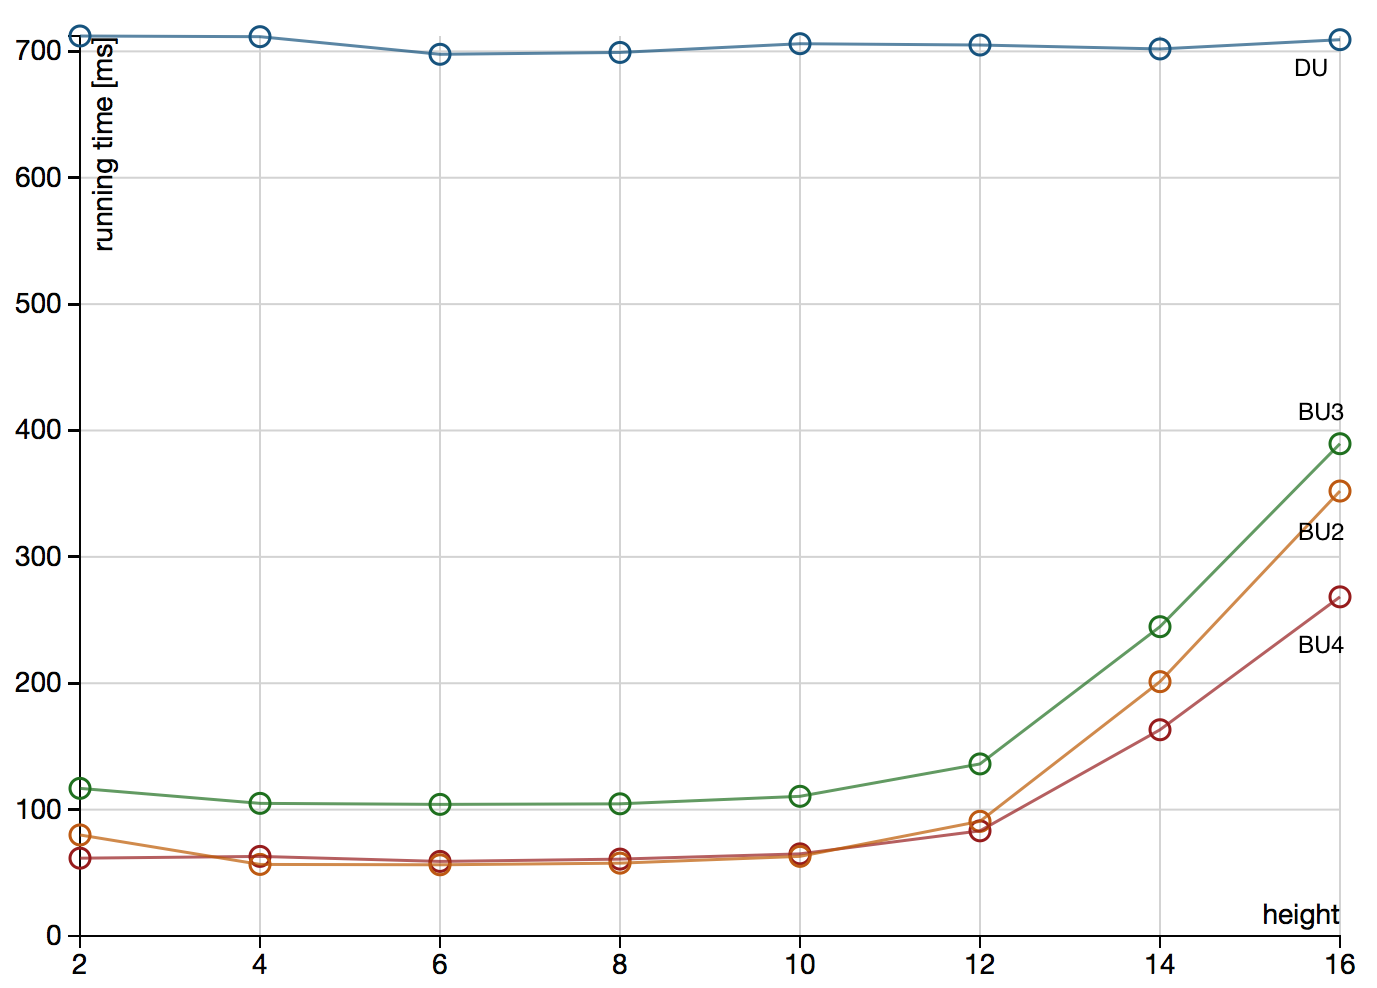
\includegraphics[width=.95\linewidth]{incremental_16_App_x1_xn_labeled}
  \caption{Incremental performance on $\treegen{\textsf{app}}{16}{x_1 \dots x_n}$ for changes of size $2^k-1$.}
  \label{fig:performance:incremental:graph}
\end{figure}

\begin{figure}[t]
  \centering
  \begin{tabular}[t]{l@{\hskip.5em}r@{\hskip1em}r@{\hskip1em}r@{\hskip1em}r@{\hskip1em}r}
    \toprule
    Tree & DU & BU2 & BU3 & BU4 \\
    \midrule
    {\scriptsize$\treegen{+}{16}{1 \ldots n}$}      & 1525.09  & 14685.65 (9.63)  & 14120.31 (9.26)  & 16221.40 (10.63) \\
    {\scriptsize$\treegen{+}{16}{x \ldots x}$}      &  1090.05  &  7678.81 (7.04)  & 8706.81 (7.99)  &  8612.78 (7.90) \\
    {\scriptsize$\treegen{+}{16}{x_1 \ldots x_n}$}  &  290.43  & 1372.44 (4.73)  & 950.32 (3.27)  & 1442.26 (4.97) \\
    \midrule                          
    {\scriptsize$\treegen{\textsf{app}}{16}{1 \ldots n}$}      &  176.32  & 2063.85 (11.71)  & 1657.92 (9.40) &  2253.84 (12.78) \\
    {\scriptsize$\treegen{\textsf{app}}{16}{x \ldots x}$}      &  171.88  &  823.60 (4.79)  &  728.33 (4.24) &  721.23 (4.20)  \\
    {\scriptsize$\treegen{\textsf{app}}{16}{x_1 \ldots x_n}$}  &   92.93  &  909.07 (9.78)  & 540.42 (5.82) &  927.04 (9.98) \\
    \midrule
    {\scriptsize overall performance} & 557.78 & 4588.90 (8.23) & 4450,69 (7.98) & 5029,76 (9.02) \\
    \bottomrule
  \end{tabular}
  \caption{Incremental performance in nodes per millisecond (speedup relative to
    DU).}
  \label{fig:performance:incremental}
\end{figure}



\paragraph{Incremental performance.}
Figure~\ref{fig:performance:incremental:graph} shows the incremental performance
of DU (blue), BU2 (orange), BU3 (green), and BU4 (red) on
$\treegen{\textsf{app}}{16}{x_1 \dots x_n}$. The x-axis shows the height of the
invalidated subexpression; the y-axis shows the run time of the four type
checkers. DU does not support incremental type checking and therefore takes the
same time to recheck the input of size $2^{16}-1$ independent of the size of the
invalidated subexpression. In contrast, BU2, BU3, and BU4 run considerably
faster. Especially for small changes, incremental type checking provides large
speedups.

Figure~\ref{fig:performance:incremental} presents a bigger picture of the
incremental performance, where we report the mean performance over all height
configurations $k$. Since DU does not support incremental type checking, it has
to recheck the whole syntax tree nonincrementally for every change.  The numbers
for DU differ from the numbers reported in
Figure~\ref{fig:performance:nonincremental} because we fixed the height to
$h=16$. For the co-contextual type checkers, we see a significant performance
improvement of up to $12.78\textsf{x}$. Incremental type checking also achieves
good speedups when all leaves refer to the same variable, which yielded
slowdowns in the nonincremental case. Furthermore, note that the reported
incremental speedups correspond to type checking after a single change to the
syntax tree. For a sequence of changes, the speedup accumulates
multiplicatively. For example, when type checking after each of 10 subsequent
changes, BU4 yields a speedup of $90.2\textsf{x}$ on average.


\section{Related work}
\label{sec:related}

% We separately discuss work related to our co-contextual formulation of type
% rules and work related to incremental type checking.

Co-contxtual type rules are different from type inference, because type
inference relies on the context to coordinate the types of
variables~\cite{Milner78}. That is, type inference assigns all references to
the same bound variable the same type. In contrast, co-contextual type checking
assigns each variable reference a fresh type and coordinates them through
requirement merging.

Our co-contextual formulation of type rules is related to prior work on
principal typing~\cite{Jim96,Wells02}, not to be confused with principal
types. A principal typing of some expression is a derivation that subsumes all
other derivations. Specifically, a principal typing (if it exists) requires the
weakest context and provides the strongest type possible for the given
expression. Principal typing finds application in type inference where, similar
to our work, the minimal context requirements can be inferred automatically. We
extend the work on principal typing by identifying the dualism between contexts
and context requirements as a method for systematically constructing
co-contextual type systems. Such a method has not been formulated in previous
work. Moreover, prior work on principal typing only considered ad-hoc
incrementalization for type checking top-level definitions, whereas we describe
a method for efficient fine-grained incremental type checking.

Other formulations of type systems related to our co-contextual one have also
been used in the context of compositional compilation~\cite{AnconaDDZ05} and the
compositional explanation of type errors~\cite{Chitil01}. However, these systems
only partially eliminated the context. In the work on compositional
compilation~\cite{AnconaDDZ05}, type checking within a module uses a standard
contextual formulation that coordinates the types of parameters and object
self-references \textsf{this}. For references to other modules, the type checker
generates constraints that are resolved by the linker. Using our method for
constructing co-contextual type systems, we can generalize this type system to
eliminate the local context as well, thus enabling compositional compilation for
individual methods.
%
In the work on compositional explanations of type errors~\cite{Chitil01}, only
the context for monomorphic variables is eliminated, whereas a context for
polymorphic variables is propagated top-down. Our extension for parametric
polymorphism demonstrated that our co-contextual formulation of type rules can
support polymorphic variables and eliminate the context entirely.

There has been surprisingly little prior work on incremental type
checking. Meertens describes an incremental type checker for the programming
language B~\cite{Meertens83}; it collects fine-grained type requirements, but is not clear on
requirement merging and also does not solve type requirements
incrementally. Johnson and Walz describe a contextual type
checker that incrementally normalizes type constraints while type checking a
program in order to precisely identify the cause of type
errors~\cite{JohnsonW86}. Aditya and Nikhil describe an incremental
Hindley/Milner type system that only supports incremental rechecking of
top-level definitions~\cite{AdityaN91}. Miao and Siek describe a type checker
for multi-staged programming~\cite{MiaoS10}; type checking in later stages is incremental
with respect to earlier stages, relying on the fact that types only get refined
by staging but assumptions on the type of an expression never have to be
revoked.

Wachsmuth~et~al. describe a task engine for name resolution and type
checking~\cite{WachsmuthKVGV13}. After a source file changes,
the incremental type checker generates new tasks for this file. The task engine
reuses cached task results where possible, computes tasks that have not been
seen before, and invalidates cached results that depend on tasks that have been
removed. The type checker relies on an incremental name analysis, whose tasks
are incrementally maintained by the same engine.

Eclipse's JDT performs incremental compilation through fine-grained dependency
tracking.\footnote{\url{http://eclipse.org/jdt/core/}} It evolved from IBM's
VisualAge~\cite{ChamberlandLR98}, which stores the code and configuration of a
software project in an in-memory database with separate entries for different
artifacts, such as methods, variables, or classpaths. The system tracks
dependencies between individual artifacts in order to update the compilation
incrementally. Similarly, Facebook's Flow\footnote{\url{http://flowtype.org}}
and Hack\footnote{\url{http://hacklang.org}} languages feature incremental type
checking through a background server that watches source files in order to
invalidate the type of changed files and files that are affected by them.
Unfortunately, not much information on the incremental type checkers of Eclipse
and Facebook is available, and it is not clear how to construct similar
incremental type checkers systematically.

Finally, there are general-purpose engines for incremental computations. Before
implementing incremental type checkers directly, we experimented with an
implementation of co-contextual type rules in an incremental SQL-like
language~\cite{MitschkeEKMS14}. In our experiment, the overhead of
general-purpose incrementalization was significant and too large for the
fine-grained incremental type checking that we are targeting. For this reason,
we did not further consider other general-purpose engines for incremental
computations, such as attribute grammars~\cite{DemersRT81} or self-adjusting
computations~\cite{AcarBBHT09}.


\section{Conclusions and future work}

We presented a co-contextual formulation for type rules and described a method
for systematically constructing co-contextual type systems. A co-contextual
formulation of type rules avoids coordination between subderivations, which
makes this formulation well-suited for parallel and incremental type
checking. In this paper, we focused on incremental type checking and described a
method for developing efficient incremental type checkers on top of
co-contextual type systems. In particular, we applied memoization to avoid
recomputing derivations for unchanged subexpressions. This enables fine-grained
incremental type checking.

We presented co-contextual type systems for PCF and extensions for records,
parametric polymorphism, and subtyping, and implemented corresponding
incremental type checkers. Our performance evaluation shows that co-contextual
type checking for PCF has performance comparable to standard contextual type
checking, and incrementalization can improve performance significantly.

In future work, we want to explore parallel type checking based on a
co-contextual formulation of type rules. Besides avoiding coordination for
generating fresh type variables, parallelization also requires efficient
strategies for distributing the syntax tree to and collecting the subresults
from multiple workers while keeping the coordination overhead minimal.

Moreover, we are currently developing a co-contextual type system for Java,
which involves complicated type rules and elaborate context requirements on
field types and method signatures. This development will lead to a fine-grained
incremental type checker for Java and will provide insights into the scalability
and applicability of our approach.


% \paragraph{\ackname} We thank Klaus Ostermann, Greg Morrisett,
% Tillmann Rendel, Guido Salvaneschi,
% and the anonymous reviewers for helpful feedback.


\bibliographystyle{abbrv}
\bibliography{bib}

\clearpage
\appendix

\section{Equivalence of contextual and co-contextual PCF}
\label{sec:appendix}

This appendix is optional and not intended for the final publication.

Recall that we call a syntactic entity ground if it does not contain unification
variables and we write $\Gamma \supseteq \reqs$ if $\Gamma(x) = \reqs(x)$ for
all $x \in \dom{\reqs}$.


\begin{lemma}
\label{lem:merge-cons}
  Let $\reqmerge{R_1}{R_2}=R|_C$, $\Gamma \supseteq \sigma_1(R_1)$, $\Gamma
  \supseteq \sigma_2(R_2)$, and $\sigma_1(R_1)$ and $\sigma_2(R_2)$ be ground.
  Then $\sigma_1\circ\sigma_2$ solves $C$.
\end{lemma}
\begin{proof}
  By the definition of \reqmergeF, $C = \{R_1(x) = R_2(x) \WHERE x \in \dom{\reqs_1} \cap \dom{\reqs_2}\}$.
%
  Since $\Gamma \supseteq \sigma_i(R_i)$, we know $\Gamma(x) = \sigma_i(R_i(x))$ for all $x \in \dom{R_i}$.
%
  In particular, $\Gamma(x)=\sigma_1(R_1(x))=\sigma_2(R_2(x))$ for all $x \in \dom{R_1}\cap\dom{R_2}$.
%
  Thus, $\sigma_1\circ\sigma_2$ solves $C$ because
  $(\sigma_1\circ\sigma_2)(R_1(x))=\sigma_1(R_1(x))=\sigma_2(R_2(x))=(\sigma_1\circ\sigma_2)(R_2(x))$ for all $x \in \dom{R_1}\cap\dom{R_2}$, because 
  $\sigma_1(R_1)$ and $\sigma_2(R_2)$ are ground.
\end{proof}

\begin{customtheorem}{\ref{thm:equiv}}[Equivalence of contextual PCF and co-contextual PCF] 
The following are equivalent:
\vspace{-1ex}
\begin{enumerate}
\item[(i)] $\judgeC{\Gamma}{e}{T}{C}$ and
  $\mathit{solve}(C)=\sigma$ such that $\sigma(T)$ is ground
\item[(ii)] $\cojudge{e}{T'}{C'}{\reqs}$ and
  $\mathit{solve}(C')=\sigma'$ such that $\sigma'(T') $ and $\sigma'(\reqs)$ are ground
\end{enumerate}
\vspace{-1ex}
  If $\sigma$ and $\sigma'$ are defined, then $\sigma(T) = \sigma'(T')$ and
  $\Gamma \supseteq \sigma'(\reqs)$.
\end{customtheorem}

\begin{proof}
  We first show $(i) \Rightarrow (ii)$ by structural induction on $e$.
  \begin{itemize}
  \item Case $n$ with \judgeC{\Gamma}{n}{T}{C}.

    By inversion, $T=\TNum$ and $C=\emptyset$.

    We choose $T'=\TNum$, $C'=\emptyset$, $R=\emptyset$, and $\sigma'=\emptyset$.

    Then $\cojudge{e}{T'}{C'}{R}$ holds, $\sigma(T)=\TNum=\sigma'(T')$,
    $\Gamma \supseteq \emptyset = \sigma'(R)$, and
    $\sigma'(T')$ and $\sigma'(R)$ are ground.


    \vskip1ex
  \item Case $x$ with \judgeC{\Gamma}{x}{T}{C}.

    By inversion, $\Gamma(x)=T$ and $C=\emptyset$.

    We choose $T'=U$, $C'=\emptyset$, $R=\{x\ofType U\}$, and $\sigma'=\{U \smap T\}$.

    Then $\cojudge{e}{T'}{C'}{R}$ holds, $\sigma(T)=T=\sigma'(U)=\sigma'(T')$,
    $\Gamma \supseteq \{x \ofType
    T\} = \sigma'(R)$,
    $\sigma'(T')$ and $\sigma'(R)$ are ground because T is ground.


    \vskip1ex
  \item Case $\abs{x}{T_1}{e}$ with \judgeC{\Gamma}{\abs{x}{T_1}{e}}{T}{C}.
    
    By inversion, \judgeC{\ctxplus{x \ofType T_1}{\Gamma}}{e}{T_2}{C_e}, $T=T_1 \to T_2$, and $C=C_e$.

    Let $\mathit{solve}(C)=\sigma$.

    By IH, \cojudge{e}{T'_2}{C'_e}{R_e} with $\mathit{solve}(C'_e)=\sigma'_e$,
    $\sigma_e(T_2)=\sigma'_e(T'_2)$, $(\ctxplus{x \ofType T_1}{\Gamma})
    \supseteq \sigma'_e(R_e)$, $\sigma'_e(T'_2)$ is ground, and
    $\sigma'_e(R_e)$ is ground. %

    We choose $T'=T_1 \to T'_2$ and $R = R_e - x$.

    \begin{itemize}
    \item If $x \in \dom{R_e}$, then $R_e(x) = U_e$ for some $U_e$. We choose
      $C' = C'_e \cup \{T_1 = R_e(x)\}$ and $\sigma'=\sigma'_e\circ\{U_e \smap T_1\}$.
      
      Then $\cojudge{e}{T'}{C'}{R}$ holds and $\sigma'$ solves $C'_e$ and $\sigma'(T_1)=T_1=\sigma'(U_e)=\sigma'(R_e(x))$.
      Moreover, $\sigma(T)=T_1 \to \sigma(T_2) = T_1 \to \sigma'(T'_2) = \sigma'(T')$,
      $\Gamma \supset \sigma'(R_e - x)$,
      $\sigma'(T')$ is ground because $T_1$ and $\sigma'(T'_2)$ are ground,
      and $\sigma'(R)$ is ground because $\sigma'_e(R_e)$ is ground.
    \item If $x \not\in \dom{R_e}$, we choose $C' = C'_e$ and $\sigma'=\sigma'_e$.

      Then $\cojudge{e}{T'}{C'}{R}$ holds, $\sigma'$ solves $C'$, $\sigma(T)=T_1 \to \sigma(T_2) = T_1 \to \sigma'(T'_2) =
      \sigma'(T')$, $\Gamma \supset \sigma'(R_e - x)$, 
      $\sigma'(T')$ is ground because $T_1$ and $\sigma'(T'_2)$ are ground,
      and $\sigma'(R)$ is ground because $\sigma'_e(R_e)$ is ground.
    \end{itemize}


    \vskip1ex
  \item Case $\app{e_1}{e_2}$ with \judgeC{\Gamma}{\app{e_1}{e_2}}{T}{C}.

    By inversion, \judgeC{\Gamma}{e_1}{T_1}{C_1}, \cojudge{\Gamma}{e_2}{T_2}{C_2}, $T=U$, and %
    $C = C_1 \cup C_2 \cup \{T_1=T_2\to U\}$.

    Let $\mathit{solve}(C)=\sigma$, which also solves $C_1$, $C_2$, and $T_1 =
    T_2 \to U$ such that $\sigma(U)$ is ground. %

    By IH for $i\in\{1,2\}$, \cojudge{e_i}{T'_i}{C'_i}{R_i} with
    $\mathit{solve}(C'_i)=\sigma'_i$, $\sigma(T_i)=\sigma'(T'_i)$, 
    $\Gamma \supseteq \sigma'_i(R_i)$, $\sigma'_i(T'_i)$ is ground, and $\sigma'_i(R_i)$ is ground. %

    Let $\reqmerge{R_1}{R_2}=R|_{C'_r}$.
    We choose $T'=U$, $C'=C'_1 \cup C'_2 \cup \{T'_1=T'_2\to U\} \cup C'_r$, and $\sigma' = \sigma'_1\circ\sigma'_2\circ\{U \smap \sigma(U)\}$.
 
    Then \cojudge{\app{e_1}{e_2}}{T'}{C'}{R} holds and $\sigma'$ solves $C'$ because it solves $C'_1$, $C'_2$, $C'_r$ (by Lemma~\ref{lem:merge-cons}), and
    $\sigma'(T'_1)=\sigma(T_1)=\sigma(T_2)\to\sigma(U)=\sigma'(T'_2)\to\sigma'(U)=\sigma'(T'_2 \to U)$.

    Moreover, $\sigma'(T')=\sigma'(U)=\sigma(U)=\sigma(T)$, 
    $\Gamma \supseteq \sigma'(R_1) \cup \sigma'(R_2) \supseteq \sigma'(R)$ by the definition of \reqmergeF,
    $\sigma'(T')$ is ground because $\sigma(U)$ is ground, and $\sigma'(R)$ is ground because $\sigma'_i(R_i)$ are ground.

    \vskip1ex
  \item Case $\add{e_1}{e_2}$ with \judgeC{\Gamma}{\add{e_1}{e_2}}{T}{C}.

    By inversion, \judgeC{\Gamma}{e_1}{T_1}{C_1}, \cojudge{\Gamma}{e_2}{T_2}{C_2}, $T=\TNum$, and %
    $C = C_1 \cup C_2 \cup \{T_1=\TNum,T_2=\TNum\}$.

    Let $\mathit{solve}(C)=\sigma$, which also solves $C_1$, $C_2$,$T_1=\TNum$, and $T_2=\TNum$. %

    By IH for $i\in\{1,2\}$, \cojudge{e_i}{T'_i}{C'_i}{R_i} with
    $\mathit{solve}(C'_i)=\sigma'_i$, $\sigma_i(T_i)=\sigma'(T'_i)$, 
    $\Gamma \supseteq \sigma'(R_i)$, $\sigma'(T'_i)$ is ground, and $\sigma'(R_i)$
    is ground. %

    Let $\reqmerge{R_1}{R_2}=R|_{C'_r}$.
    We choose $T'=\TNum$, $C'=C'_1 \cup C'_2 \cup \{T'_1=\TNum,T'_2=\TNum\} \cup C'_r$, and $\sigma' = \sigma'_1\circ\sigma'_2$.

    Then \cojudge{\add{e_1}{e_2}}{T'}{C'}{R} and $\sigma'$ solves $C'$ because it solves $C'_1$, $C'_2$, $C'_r$ (by Lemma~\ref{lem:merge-cons}), and
    $\sigma'(T'_i)=\sigma(T_i)=\TNum$.

    Moreover, $\sigma'(T')=\TNum=\sigma(T)$,
    $\Gamma \supseteq \sigma'(R_1) \cup \sigma'(R_2) \supseteq \sigma'(R)$ by the definition of \reqmergeF,
    $\sigma'(T')=\TNum$ is ground, and $\sigma'(R)$ is ground  because $\sigma'_i(R_i)$ are ground.

  \vskip1ex
\item Case $\ifzero{e_1}{e_2}{e_3}$ with \judgeC{\Gamma}{\ifzero{e_1}{e_2}{e_3}}{T}{C}.%

  By inversion for $i\in\{1,2,3\}$, \judgeC{\Gamma}{e_i}{T_i}{C_i}, $T=T_2$, and%
   $C=C_1 \cup C_2 \cup C_3 \cup \{T_1=\TNum, T_2=T_3\}$.
  
  Let $\mathit{solve}(C)=\sigma$, which also solves $C_1$, $C_2$, $C_3$, $T_1 = \TNum$, and $T_2 = T_3$. %

  By IH, \cojudge{e_i}{T'_i}{C'_i}{R_i} with 
  $\mathit{solve}(C'_i) = \sigma'_i$, $\sigma'_i(T'_i)=\sigma(T_i)$,
  $\Gamma\supseteq \sigma'_i(R_i)$, $\sigma'(T'_i)$ is ground, and $\sigma'(R_i)$
    is ground. %

  Let $\reqmerge{R_2}{R_3}=R_{2,3}|_{C'_{2,3}}$, $\reqmerge{R_1}{R_{2,3}}=R_{1,2,3}|_{C'_{1,2,3}}$.
  We choose $R=R_{1,2,3}$, %
  $T' = T'_2$,
  $C'=C'_1 \cup C'_2 \cup C'_3 \cup \{T'_1=\TNum, T'_2=T'_3\} \cup C'_{2,3} \cup C'_{1,2,3}$, and $\sigma=\sigma_1\circ\sigma_2\circ\sigma_3$.

  Then \cojudge{\ifzero{e_1}{e_2}{e_3}}{T'}{C'}{R} and $\sigma'$ solves $C'$ because it solves
  $C'_1$, $C'_2$,$C'_3$, $C'_{2,3}$ (by Lemma~\ref{lem:merge-cons}), $C'_{1,2,3}$ (by Lemma~\ref{lem:merge-cons}), 
  and $\sigma'(T'_1)=\sigma(T_1)=\TNum$ as well as $\sigma'(T'_2)=\sigma(T_2)=\sigma(T_3)=\sigma'(T'_3)$.

  Moreover, $\sigma'(T')=\sigma'(T'_2)=\sigma(T_2)=\sigma(T)$,
  $\Gamma \supseteq \sigma'(R_1) \cup \sigma'(R_2) \cup \sigma'(R_3) \supseteq \sigma'(R_1) \cup \sigma'(R_{2,3}) \supseteq \sigma'(R_{1,2,3})$ by the definition of \reqmergeF, 
  $\sigma'(T')$ is ground because $\sigma'(T'_2)$ is ground, and $\sigma'(R)$ is ground  because $\sigma'_i(R_i)$ are ground.  
      
    \vskip1ex
  \item Case $\fix{e}$ with \judgeC{\Gamma}{\fix{e}}{T}{C}.

    By inversion, \judgeC{\Gamma}{e}{T_e}{C_e}, $T=U$, and $C=C_e \cup \{T_e=U \to U\}$.

  Let $\mathit{solve}(C)=\sigma$, which solves $C_e$ and $T_e=U \to U$ such that $\sigma(U)$ is ground.

    By IH, \cojudge{e}{T'_e}{C'_e}{R_e} with
    $\mathit{solve}(C'_e)=\sigma'_e$, $\sigma'_e(T'_e)=\sigma(T_e)$, $\Gamma_e
    \supseteq \sigma'(R_e)$, $\sigma'(T'_e)$ is ground, and $\sigma'(R_e)$
    is ground.

    We choose $R = R_e$, $T'=U$, $C' = C'_e \cup \{T'_e=U \to U\}$, and $\sigma'=\sigma'_e\circ\{U \smap \sigma(U)\}$.

    Then \cojudge{\fix{e}}{T'}{C'}{R} and $\sigma'$ solves $C'$ because it
    solves $C'_e$ and $\sigma'(T'_e)=\sigma(T_e)=\sigma(U \to U) =
    \sigma(U)\to\sigma(U)=\sigma'(U)\to\sigma'(U)=\sigma'(U \to U)$.
    
    Moreover, $\sigma'(T')=\sigma'(U)=\sigma(U)=\sigma(T)$,
    $\Gamma=\Gamma_e\supseteq \sigma'(R_e) = \sigma'(R)$,
    $\sigma'(T')$ is ground because $\sigma(U)$ ground, and $\sigma'(R)$ is ground because $\sigma'(R_e)$ is ground.
%
  \end{itemize}


\noindent  Next we show $(ii) \Rightarrow (i)$ by structural induction on $e$.

  \begin{itemize}
  \item Case $n$ with \cojudge{n}{T'}{C'}{\reqs}. %

    By inversion, $T'=\TNum$, $C'=\emptyset$, and $\reqs=\emptyset$. %

    Let $\mathit{solve}(C')=\sigma'$.
    We choose $\Gamma=\emptyset$, $T=\TNum$, $C=\emptyset$, $\sigma=\emptyset$. 

    Then \judgeC{\Gamma}{e}{T}{C} holds, $\sigma(T)=\TNum=\sigma'(T')$, $\Gamma = \emptyset = \sigma'(\reqs)$, and $\sigma(T)$ is ground.

    \vskip1ex
  \item Case $x$ with \cojudge{x}{T'}{C'}{\reqs}. %

    By inversion, $T'=U$, $C'=\emptyset$, and $\reqs=\{x \ofType U\}$.

    Let $\sigma'(U) = T_x$ for some $T_x$ that we know is ground. %

    We choose $\Gamma=\ctxplus{x\ofType T_x}{\emptyset}$, $T=T_x$, $C=\emptyset$, and $\sigma=\emptyset$.

    Then \judgeC{\Gamma}{e}{T}{C} holds, %
    $\sigma(T)=T_x=\sigma'(U)$,%
    $\Gamma = (\ctxplus{x\ofType T_x}{\emptyset}) \supseteq \{x\ofType T_x\} = \sigma'(\reqs)$, and
    $\sigma(T)$ is ground because $T_x$ is ground. %

    \vskip1ex
\item Case $\abs{x}{T_1}{e}$ with \cojudge{\abs{x}{T_1}{e}}{T'}{C'}{R}. %

  By inversion, \cojudge{e}{T'_2}{C'_e}{R_e}, $T'=T_1\to T'_2$, and $R = R_e - x$ for some $T'_2$, $C'_e$, and $R_e$. %

  Let $\mathit{solve}(C')=\sigma'$, which also solves $C'_e$. %

  By IH, \judgeC{\Gamma_e}{T_2}{e}{C_e} with $\mathit{solve}(C_e)=\sigma_e$,
  $\sigma_e(T_2)=\sigma'(T'_2)$, $\Gamma_e \supseteq \sigma'(R_e)$, and $\sigma_e(T_2)$ is ground. %
%
  The latter entails $\Gamma_e(x) = \sigma'(R_e(x))$ for all $x \in \dom{R_e}$. %

  We choose $T=T_1\to T_2$, $C=C_e$, and $\sigma=\sigma_e$ such that
  $\sigma(T)=T_1\to \sigma(T_2) = T_1 \to \sigma'(T'_2) = \sigma'(T')$ and $\sigma(T)$ is ground because $T_1$ and $\sigma_e(T_2)$ are ground.

  \begin{itemize}
  \item If $x \in \dom{R_e}$, %
    then $(T_1=R_e(x)) \in C'$ and $T_1=\sigma'(R_e(x)) = \Gamma_e(x)$. %
    Thus, by swapping $\Gamma_e=(\ctxplus{x \ofType T_1}{\Gamma})$ for some $\Gamma$
    such that \judgeC{\Gamma}{e}{T}{C} holds,
    $\sigma$ solves $C$, and
    $\Gamma \supseteq \Gamma_e - x \supseteq \sigma'(R_e) - x = \sigma'(R_e - x)$.
  \item If $x \not\in \dom{R_e}$, the $x$ is not free in $e$ and %
    we get \judgeC{\ctxplus{x \ofType T_1}{(\Gamma_e - x)}}{T_2}{e}{C_e} by strengthening and weakening. %
    We choose $\Gamma = \Gamma_e - x$ such that (i) holds and %
    $\Gamma = \Gamma_e - x \supseteq \sigma'(R_e) - x = \sigma'(R_e - x)$.
  \end{itemize}

    \vskip1ex
\item Case $\app{e_1}{e_2}$ with \cojudge{\app{e_1}{e_2}}{T'}{C'}{R}. %

  By inversion, \cojudge{e_1}{T'_1}{C'_1}{R_1}, \cojudge{e_2}{T'_2}{C'_2}{R_2}, $\reqmerge{R_1}{R_2}=R|_{C'_r}$, $T'=U$, and %
  $C' = C'_1 \cup C'_2 \cup \{T'_1=T'_2\to U\} \cup C'$.

  Let $\mathit{solve}(C')=\sigma'$, which also solves $C'_1$, $C'_2$, $C'_r$, and $T'_1 = T'_2 \to U$ such that $\sigma'(U)$ is ground. %

  By IH for $i\in\{1,2\}$, \judgeC{\Gamma_i}{e_i}{T_i}{C_i} with
  $\mathit{solve}(C_i)=\sigma_i$, $\sigma_i(T_i)=\sigma'(T'_i)$, 
  $\Gamma_i \supseteq \sigma'(R_i)$, and
  $\sigma_i(T_i)$ is ground. %

  We choose  $\Gamma=\ctxplus{\Gamma_1}{\Gamma_2}$, $T=U$, %
  $C = C_1 \cup C_2 \cup \{T_1=T_2\to U\}$, and $\sigma=\sigma_1 \circ \sigma_2 \circ \{U \smap \sigma'(U)\}$. 

  Since $\sigma_i(\Gamma_i) \supseteq \sigma'(R_i)$, $\Gamma$ only extends %
  $\Gamma_1$ and $\Gamma_2$ with variables that are not free in $e_1$ and $e_2$, respectively.%
%
  Thus, \judgeC{\Gamma}{e_i}{T_i}{C_i} and \judgeC{\Gamma}{\app{e_1}{e_2}}{U}{C}.
  $\sigma$ solves $C$ because it solves $C_1$ and $C_2$ and $\sigma(T_1)=\sigma'(T'_1)=\sigma'(T'_2 \to U)=\sigma'(T'_2)\to\sigma'(U)=\sigma(T_2)\to\sigma(U)=\sigma(T_2\to U)$.

  Moreover, 
  $\sigma(T)=\sigma(U)=\sigma'(U)=\sigma'(T')$,
  $\Gamma=\ctxplus{\Gamma_1}{\Gamma_2} \supseteq \sigma'(R_1) \cup \sigma'(R_2) \supseteq \sigma'(R)$ by the definition of \reqmergeF,
  and $\sigma(T)$ is ground because $\sigma'(U)$ is ground.

    \vskip1ex
\item Case $\add{e_1}{e_2}$ with \cojudge{\add{e_1}{e_2}}{T'}{C'}{R}. %

  By inversion for $i\in\{1,2\}$, \cojudge{e_i}{T'_i}{C'_i}{R_i}, $\reqmerge{R_1}{R_2}=R|_{C'_r}$, $T'=\TNum$, and %
  $C' = C'_1 \cup C'_2 \cup \{T'_1=\TNum, T'_2=\TNum\} \cup C'_r$.

  Let $\mathit{solve}(C')=\sigma'$, which also solves $C'_1$, $C'_2$, $C'_r$, $T'_1 = \TNum$, and $T'_2 = \TNum$. %

  By IH, \judgeC{\Gamma_i}{e_i}{T_i}{C_i} with
  $\mathit{solve}(C_i)=\sigma_i$, $\sigma_i(T_i)=\sigma'(T'_i)$, 
  $\Gamma_i \supseteq \sigma'(R_i)$,
  and $\sigma_i(T_i)$ is ground. %

  We choose $\Gamma=\ctxplus{\Gamma_1}{\Gamma_2}$, $T=\TNum$, %
  $C = C_1 \cup C_2 \cup \{T_1=\TNum, T_2=\TNum\}$, and $\sigma=\sigma_1\circ\sigma_2$.

  Since $\sigma_i(\Gamma_i) \supseteq \sigma'(R_i)$, $\Gamma$ only extends %
  $\Gamma_1$ and $\Gamma_2$ with variables that are not free in $e_1$ and $e_2$, respectively.%
  %
  Thus, \judgeC{\Gamma}{e_i}{T_i}{C_i} and \judgeC{\Gamma}{\add{e_1}{e_2}}{\TNum}{C}.

  $\sigma$ solves $C$ because it solves $C_1$ and $C_2$ and $\sigma(T_i)=\sigma'(T'_i)=\TNum$.

  Moreover, 
  $\sigma(T)=\TNum=\sigma'(T')$,
  $\Gamma=\ctxplus{\Gamma_1}{\Gamma_2} \supseteq \sigma'(R_1) \cup \sigma'(R_2) \supseteq \sigma'(R)$ by the definition of \reqmergeF,
  and $\sigma(T)=\TNum$ is ground.  

    \vskip1ex
\item Case $\ifzero{e_1}{e_2}{e_3}$ with \cojudge{\ifzero{e_1}{e_2}{e_3}}{T'}{C'}{R}.%

  By inversion for $i\in\{1,2,3\}$, \cojudge{e_i}{T'_i}{C'_i}{R_i}, %
  $\reqmerge{R_2}{R_3}=R_{2,3}|_{C_{2,3}}$, $\reqmerge{R_1}{R_{2,3}}=R_{1,2,3}|_{C_{1,2,3}}$, %
  $T' = T$, $R=R_{1,2,3}$, and %
  $C'=C'_1 \cup C'_2 \cup C'_3 \cup \{T'_1=\TNum, T'_2=T'_3\} \cup C_{2,3} \cup C_{1,2,3}$.

  Let $\mathit{solve}(C')=\sigma'$, which also solves $C'_1$, $C'_2$, $C'_3$, $C_{2,3}$, $C_{1,2,3}$, $T'_1 = \TNum$, and $T'_2 = T'_3$. %

  By IH, \judgeC{\Gamma_i}{e_i}{T_i}{C_i} with 
  $\mathit{solve}(C_i) = \sigma_i$, $\sigma_i(T_i)=\sigma'(T'_i)$, $\Gamma_i \supseteq \sigma'(R_i)$, and $\sigma_i(T_i)$ is ground. %

  We choose $\Gamma=\ctxplus{\Gamma_1}{\ctxplus{\Gamma_2}{\Gamma_3}}$, $T=T_2$, %
  $C = C_1 \cup C_2 \cup C_3 \cup \{T_1=\TNum, T_2=T_3\}$, and $\sigma=\sigma_1\circ\sigma_2\circ\sigma_3$.

  Since $\sigma_i(\Gamma_i) \supseteq \sigma'(R_i)$, $\Gamma$ only extends %
  $\Gamma_1$, $\Gamma_2$, and $\Gamma_3$ with variables that are not free in $e_1$, $e_2$, and $e_3$, respectively.%
  % 
  Thus, \judgeC{\Gamma}{e_i}{T_i}{C_i} and \judgeC{\Gamma}{\ifzero{e_1}{e_2}{e_3}}{T_2}{C}.

  $\sigma$ solves $C$ because it solves $C_1$, $C_2$, and $C_3$ and $\sigma(T_1)=\sigma'(T'_1)=\TNum$ as well as $\sigma(T_2)=\sigma'(T'_2)=\sigma'(T'_3)=\sigma(T_3)$.

  Moreover,
  $\sigma(T)=\sigma_2(T_2)=\sigma'(T'_2)=\sigma'(T')$,
  $\Gamma=\ctxplus{\Gamma_1}{\ctxplus{\Gamma_2}{\Gamma_3}} \supseteq \sigma'(R_1) \cup \sigma'(R_2) \cup \sigma'(R_3) \supseteq \sigma'(R_1) \cup \sigma'(R_{2,3}) \supseteq \sigma'(R_{1,2,3})$ by the definition of \reqmergeF,
  and $\sigma(T)$ is ground because $\sigma_2(T_2)$ is ground.  

    \vskip1ex
  \item Case $\fix{e}$ with \cojudge{\fix{e}}{T'}{C'}{R}.

    By inversion, \cojudge{e}{T'_e}{C'_e}{R_e}, $T'=U$, $C'=C'_e \cup \{T'_e=U \to U\}$, and $R=R_e$.

  Let $\mathit{solve}(C')=\sigma'$, which solves $C'_e$ and $T'_e=U \to U$ such that $\sigma'(U)$ is ground.

    By IH, \judgeC{\Gamma_e}{e}{T_e}{C_e} with
    $\mathit{solve}(C_e)=\sigma_e$, $\sigma_e(T_e)=\sigma'(T'_e)$,
    $\Gamma_e \supseteq \sigma'(R_e)$,
    and $\sigma(T_e)$ is ground.

    We choose $\Gamma=\Gamma_e$, $T=U$, $C = C_e \cup \{T_e=U \to U\}$, and $\sigma=\sigma_e\circ\{U \smap \sigma'(U)\}$.

    Then \judgeC{\Gamma}{\fix{e}}{T}{C} and $\sigma$ solves $C$ because it
    solves $C_e$ and $\sigma(T_e)=\sigma'(T'_e)=\sigma'(U \to
    U)=\sigma'(U)\to\sigma'(U)=\sigma(U)\to\sigma(U)=\sigma(U \to U)$.
    Moreover, 
    $\sigma(T)=\sigma(U)=\sigma'(U)=\sigma'(T')$,
    $\Gamma=\Gamma_e\supseteq \sigma'(R_e) = \sigma'(R)$,
    and $\sigma(T)$ is ground because $\sigma'(U)$ is ground.
%
  \end{itemize}

\end{proof}

\end{document}


%%% Local Variables: 
%%% mode: latex
%%% TeX-master: t
%%% End: 
